\section{$\!\!\!\!\!\!\!$. Four Specific Cases of Ge-N$_d$ Distribution Family}    % Section S1

In the previous, we assume that the mixture variable $\tau$ follows an arbitrary parametric distribution $f_\tau(\tau|\bla)$ and construct $\GeN$ family. Now we fix $\tau$ as some specific distributions in \textit{generalized inverse Gaussian} (GIGau, see more details in \S\ref{zyf.four.S.sec:GIGau}) family (i.e., gamma, inverse gamma, inverse Gaussian and reciprocal inverse Gaussian) to explore the so-called Ga-N$_d$, IGa-N$_d$, IGau-N$_d$ and RIGau-N$_d$ distributions and study their basic properties, statistical inferences together with the corresponding mean regression models.

In order to completely eliminate the parameter coupling problem between the covariance matrix and the marginal kurtosis and ensure the identifiability, we impose the inverse expectation of mixture variable $E(\tau^{-1}) = 1$ via the scale transformation property in GIGau family.

\subsection{The gamma mixture of multivariate normal distribution}       % Section S1.1

A positive \textit{random variable} (r.v.) $Y$ is said to follow the gamma distribution with shape parameter $\al \, (>0)$ and rate parameter $\be \, (>0)$, denoted by $Y \sim \mGamma(\al, \be)$, if its \textit{probability density function} (pdf) is
\begin{eqnarray*}
    \mGamma(y | \al, \be) = \frac{\be^\al}{\Ga(\al)} y^{\al - 1} \e^{-\be y}, \quad y > 0.
\end{eqnarray*}
We have $E(Y^{-1}) = \be / (\al - 1)$ (if $\al > 1$) and $\Var(Y^{-1}) = \be^2 / [(\al - 1)^2 (\al - 2)]$ (if $\al > 2$). 

It is easy to show that if $Y \sim \mGamma(\al, \be)$, then $c \cdot Y \sim \mGamma(\al, \be/c)$ for any constant $c > 0$. Let $Z^* \sim N_d(\0, \bSi^*)$, $\tau^* \sim \mGamma(\la, \be^*)$ and $Z^* \inde \tau^*$. If we define $\ibX \sd \bmu + Z^* / \sqrt{\tau^*}$, then
\begin{eqnarray*}
    \ibX &\sd& \bmu + \frac{N_d(\0, \bSi^*)}{\mGamma(\la, \be^*)} = \bmu + \frac{N_d(\0, \bSi^*)}{\sqrt{(\la - 1) / \be^* \cdot \mGamma(\la, \la - 1)}} \\ [2mm]
    &=& \bmu + \frac{N_d(\0, \frac{\be^*}{\la - 1} \bSi^*)}{\sqrt{\mGamma(\la, \la - 1)}} = \bmu + \frac{N_d(\0, \bSi)}{\sqrt{\mGamma(\la, \la - 1)}},
\end{eqnarray*}
where $\bSi = \be^* \bSi^* / (\la - 1)$ and $\tau \sim \mGamma(\la, \la - 1)$ with $E(\tau^{-1}) = 1$ for any $\la > 1$, which can motivate the following definition.

\subsubsection{Definition and basic properties of the Ga-N$_d$ distribution}        % Section S1.1.1

\begin{definition}{\rm \textbf{(Ga-N$_d$ distribution).} Suppose that $\tau \sim \mGamma(\la, \la - 1)$ with $\la > 1$ and the \textit{stochastic representation} (SR):
$$
    \ibX \sd \bmu + \frac{\ibZ}{\sqrt{\tau}}, 
$$
where $\bmu = (\mu_1, \dots, \mu_d)^\top \in \bbR^d$ is the location parameter, $\ibZ = (Z_1, \dots, Z_d)^\top \sim N_d(\0, \bSi)$ with scale matrix $\bSi = (\sigma_{ij})_{d\times d}$ and $\ibZ \inde \tau$, then the \trv $\ibX = (X_1, \dots, X_d)^\top$ is said to follow the Ga-N$_d$ distribution, denoted by $\ibX \sim \GaN$ or Ga-N$_d(\bth)$, where $\bth = \{\bmu, \bSi, \la\}$ is the parameter vector. \hfill $\|$
}\end{definition}

By setting $f_\tau(\tau|\bla) = \mGamma(\tau|\la, \la - 1)$, we obtain the pdf of $\ibX \sim \GaN$ as
\begin{eqnarray}
    \mbox{Ga-N}_d(\ibx|\bth) &=& \frac{(\la - 1)^\la}{(2\pi)^\frac{d}{2} |\bSi|^\frac{1}{2} \Ga(\la)} \int_0^\infty h_{1*}(\tau | \ibx, \bth) \rd \tau \label{zyf.four.S1.1} \\ [2mm]
    &=& \frac{(\la - 1)^\la \Ga(\frac{d}{2} + \la)}{(2\pi)^\frac{d}{2} |\bSi|^\frac{1}{2} \Ga(\la)} \left[ \frac{(\ibx - \bmu)^\top \bSi^{-1} (\ibx - \bmu)}{2} + \la - 1 \right]^{-\frac{d}{2} - \la}, \non
\end{eqnarray}
where 
\begin{eqnarray*}
    h_{1*}(\tau | \ibx, \bth) = \tau^{\frac{d}{2} + \la - 1} \exp\left\{-\left[\frac{(\ibx - \bmu)^\top \bSi^{-1} (\ibx - \bmu)}{2} + \la - 1 \right]\tau\right\}.
\end{eqnarray*}
We easily compute the expectation, variance and kurtosis as
\begin{eqnarray*}
    E(\ibX) = \bmu, \quad \Var(\ibX) = \bSi \qand \Kurt(X_j) = \frac{3}{\la - 2}, \quad j = 1, \dots, d.
\end{eqnarray*}
\begin{remark}{\rm \textbf{(Alternative form of multivariate Students' $t$ distribution).} By observing the SR of multivariate Student's $t$ distribution
$$
    \ibX_t \sd \bmu_t + \frac{\ibZ_t}{\sqrt{\mGamma(\nu/2, \nu/2)}},
$$
where $\ibZ_t \sim N_d(\0, \bSi_t)$. We found that $\GaN$ is actually an alternative form with $\bmu = \bmu_t$, $\bSi = (1 - 2/\nu)\bSi_t$ and $\la = \nu / 2$. Therefore, in \S\ref{zyf.four.S.sec:GaN}, we will propose a new approach (i.e., the N-EM algorithm for the first time) to calculate the MLEs of Ga-N$_d$ distribution (also known as multivariate Students' $t$ distribution). \hfill $\|$
}\end{remark}
\begin{figure}[H]
    \subfigure[$\;$ $\bmu = (-0.5, -1)^\top$, $\bSi = (1, 0; 0, 2)$ and $\la = 2.5$;]
    {
        \centering
        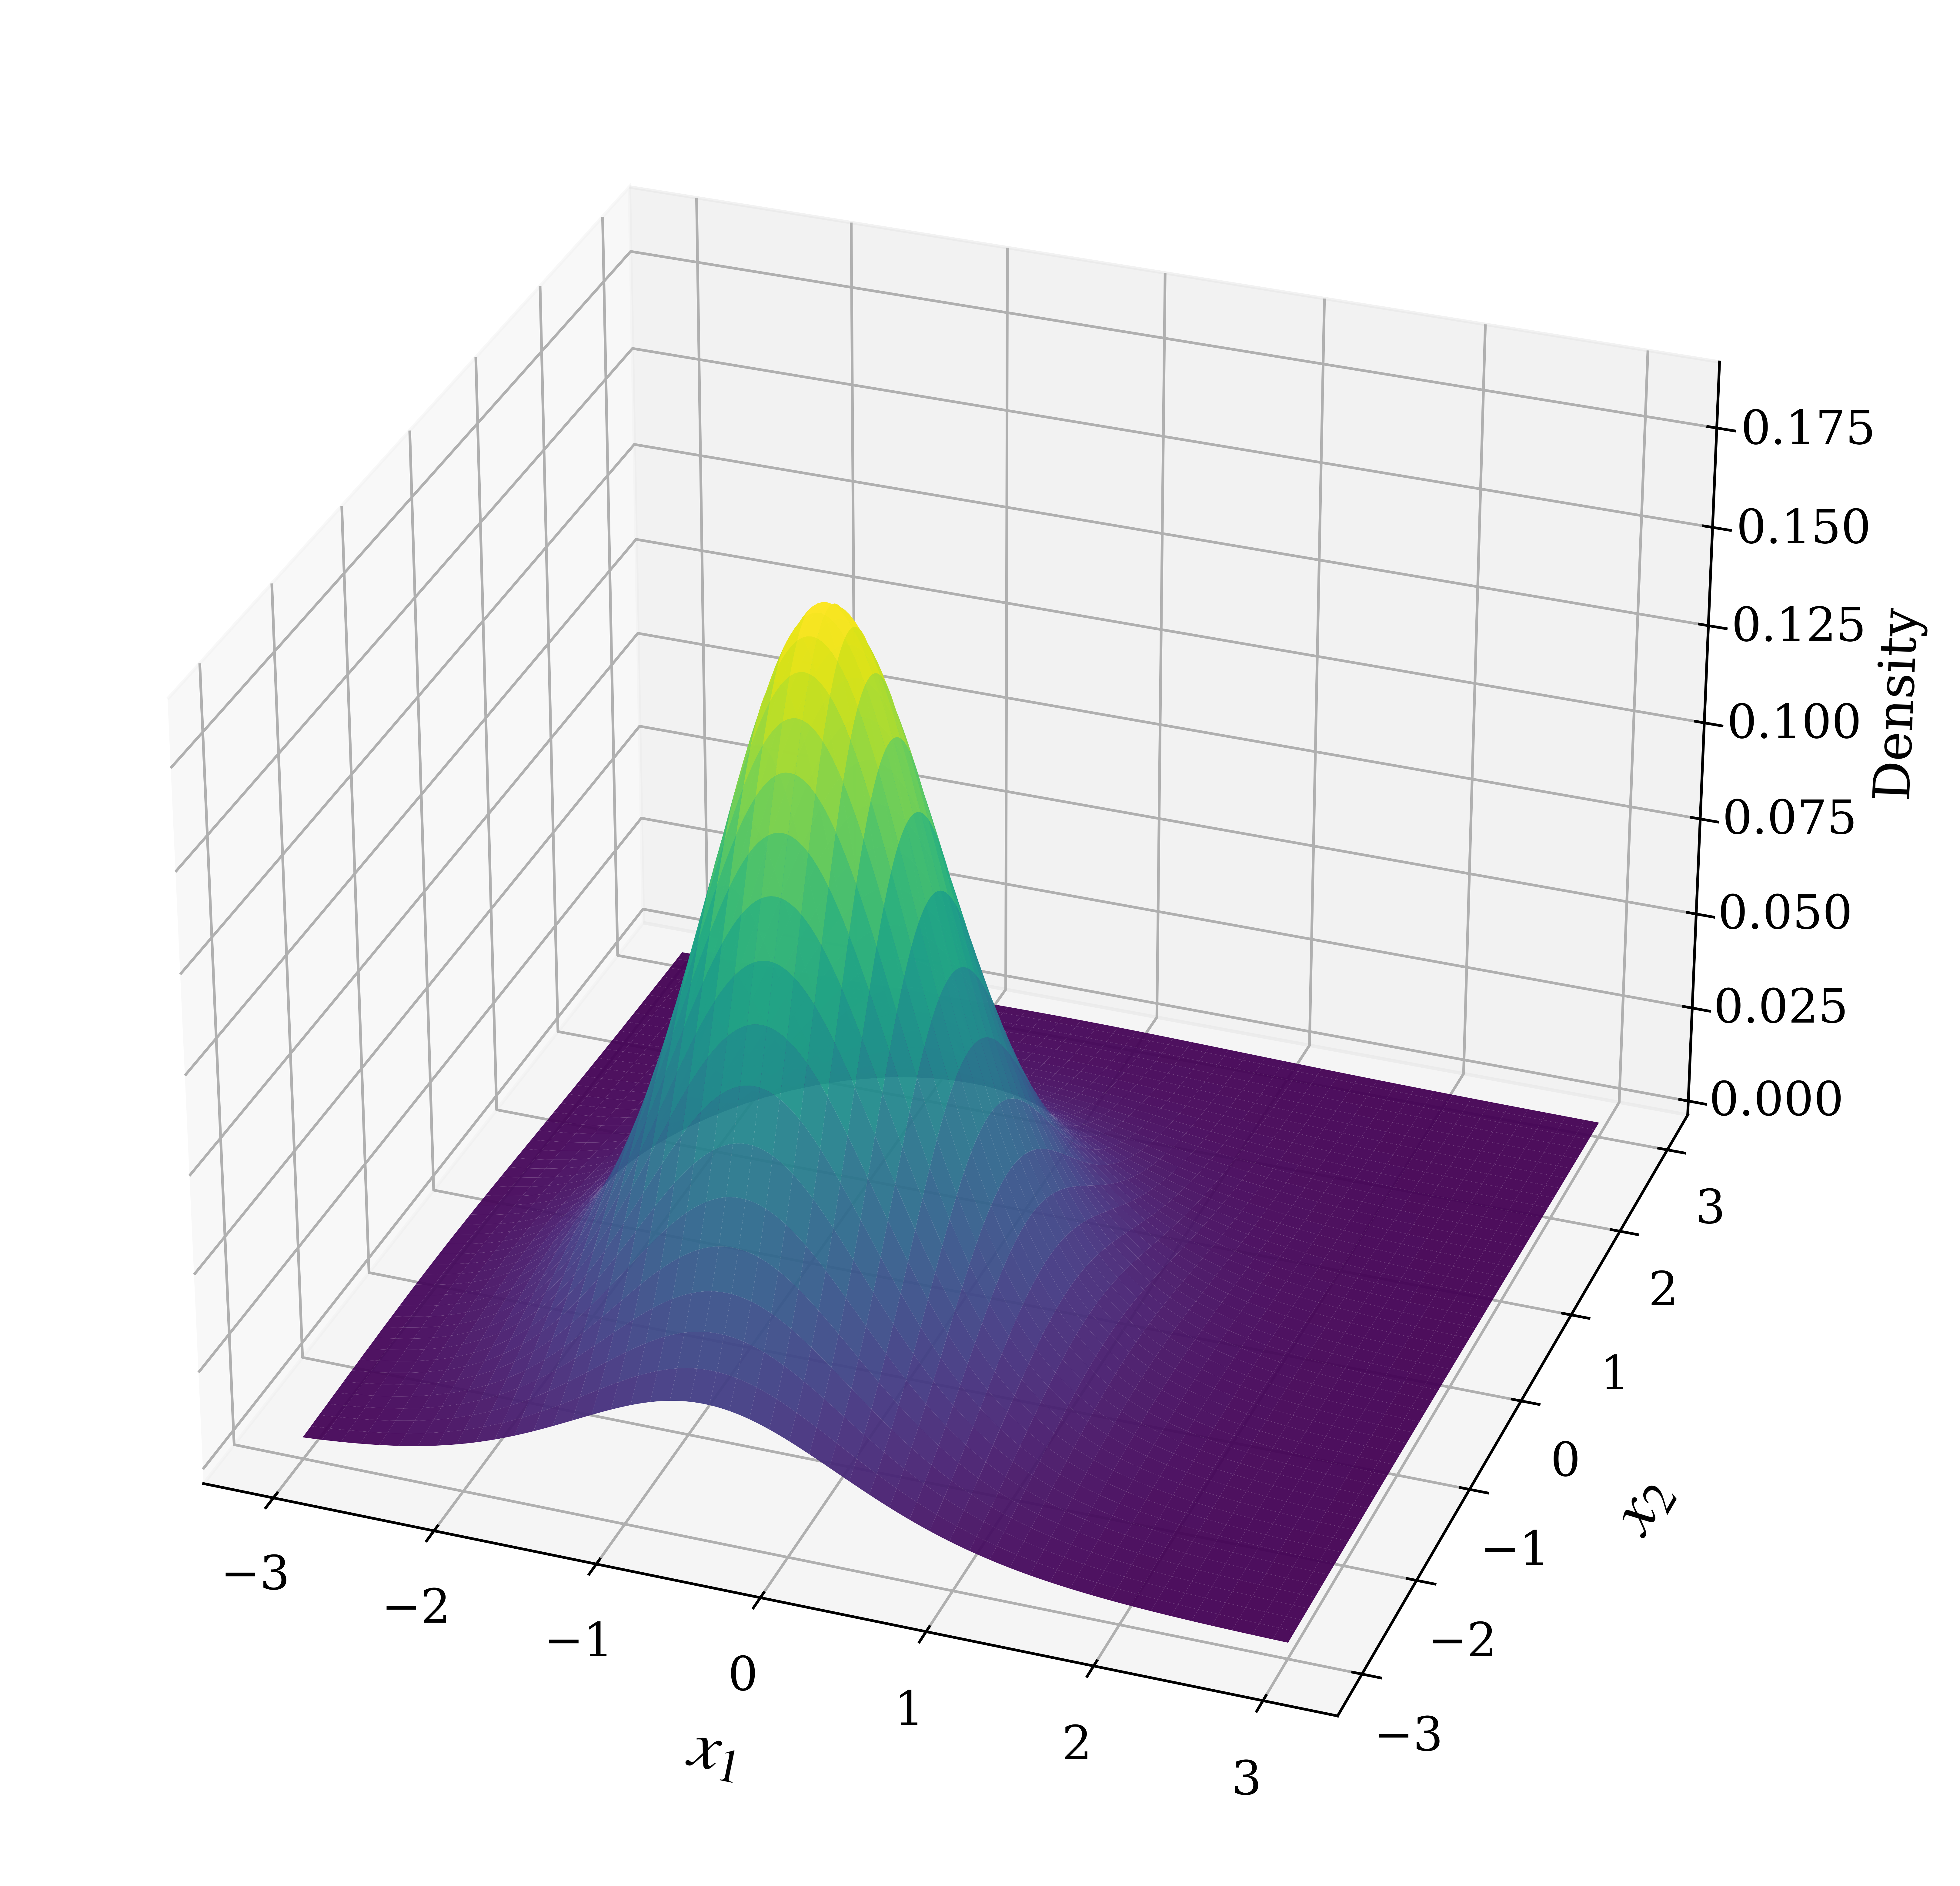
\includegraphics[width=0.5\linewidth]{figures/plot1.png}
    }
    \subfigure[$\;$ $\bmu = (0, 0)^\top$, $\bSi = (1, 0.5; 0.5, 1)$ and $\la = 2.5$;]
    {
        \centering
        
\includegraphics[width=0.5\linewidth]{figures/plot2.png}
    }
    \subfigure[$\;$ $\bmu = (0, 0)^\top$, $\bSi = (1, -0.5; -0.5, 1)$ and $\la = 3$;]
    {
        \centering
        
\includegraphics[width=0.5\linewidth]{figures/plot3.png}
    }
    \subfigure[$\;$ $\bmu = (0, 0)^\top$, $\bSi = (1, 0.5; 0.5, 1)$ and $\la = 3$.]
    {
        \centering
        
\includegraphics[width=0.5\linewidth]{figures/plot4.png}
    }
    \caption{$\;$ Density of $\GaN$ distribution with various parameter combinations.}
    \label{zyf.four.S.fig1}
\end{figure}

\subsubsection{Mean regression model and MLEs computation for $\GaN$}\label{zyf.four.S.sec:GaN}     % Section S1.1.2

Suppose that $\{\ibX_i\}_{i=1}^n \ind \mbox{Ga-N}_d(\bmu_i, \bSi, \la)$ and $\Y{obs} = \{\ibx_i, \ibzi\}_{i=1}^n$ denote the observed data, we consider the following mean regression model
$$
    E(\ibX_i | \ibzi) = \bmu_i = \bB^\top \ibzi, \quad i = 1, \dots, n, 
$$
where $\ibzi = (z_{i1}, \dots, z_{iq})^\top$ is a $q$-dimensional vector of covariates for the $i$-th subject, the matrix of regression coefficients
\begin{eqnarray*}
    \bB = \left(
    \begin{array}{cccc}
        \be_{11} & \be_{12} & \cdots & \be_{1d} \\ 
        \be_{21} & \be_{22} & \cdots & \be_{2d} \\ 
        \vdots   & \vdots   & \ddots & \vdots   \\
        \be_{q1} & \be_{q2} & \cdots & \be_{qd}
    \end{array}
    \right),
\end{eqnarray*}
with $q \times d + d(d + 1) / 2 + 1 \le n$. Let $\bga = \{ \bB, \bSi, \bla\}$ be the parameter vector, the log-likelihood function of $\bga$ is
\begin{eqnarray*}
    \ell_1(\bga | \Y{obs}) &\sr{\rm (\ref{zyf.four.S1.1})}& -\frac{nd}{2} \log(2\pi) - \frac{n}{2} \log|\bSi| + n\la\log(\la - 1) -n\log\Ga(\la) \\ [2mm]
    && +\; \sum_{i=1}^n \log \int_0^\infty h_1(\tau | \ibx_i, \ibzi, \bga) \rd \tau,
\end{eqnarray*}
where $h_1(\tau | \ibx_i, \ibzi, \bga) \teq \tau^{d/2 + \la - 1} \exp\{-[(\ibx_i - \bB^\top \ibzi)^\top \bSi^{-1} (\ibx_i - \bB^\top \ibzi)/2 + \la - 1]\tau\}$. To calculate the MLEs of $\bga$, we utilize the N-EM algorithm. By computing the \textit{normalizing density function} (ndf)
\begin{eqnarray*}
    g_1(\tau | \ibx_i, \ibzi, \bga) &\teq& \frac{h_1(\tau | \ibx_i, \ibzi, \bga)}{\int_0^\infty h_1(s | \ibx_i, \ibzi, \bga) \rd s} \\ [2mm]
    &=& \mGamma\left( \tau \;\bigg|\; \frac{d}{2} + \la,\; \frac{(\ibx_i - \bB^\top\ibzi)^\top \bSi^{-1} (\ibx_i - \bB^\top \ibzi)}{2} + \la - 1 \right),
\end{eqnarray*}
we construct the surrogate function 
\begin{eqnarray*}
    Q_1(\bga | \bgat) &=& \ct{1} - \frac{n}{2} \log|\bSi| - \frac{1}{2} \sum_{i=1}^n \at{i,1} \left(\ibx_i - \bB^\top \ibzi \right)^\top \bSi^{-1} \left(\ibx_i - \bB^\top \ibzi \right) \\ [2mm]
    && +\; n\left[\la\log(\la - 1) - \log\Ga(\la) + \left(\Bdt{1}-\Bat{1}\right)\la\right],
\end{eqnarray*}
with constant $\ct{1}$ free from $\bga$ and for $i = 1, \dots, n$, 
\begin{eqnarray*}
    && \at{i,1} = \int_0^\infty \tau \cdot g_1(\tau | \ibx_i, \ibzi, \bgat) \rd \tau, \hspace{1cm} \Bat{1} \teq \frac{1}{n} \sum_{i=1}^{n} \at{i,1}, \\ [2mm]
    && \dt{i,1} = \int_0^\infty \log\tau \cdot g_1(\tau | \ibx_i, \ibzi, \bgat) \rd \tau, \quad \Bdt{1} \teq \frac{1}{n} \sum_{i=1}^{n} \dt{i,1}.
\end{eqnarray*}
By maximizing $Q_1(\bga | \bgat)$ respect to $\bga$, we obtain the $(t+1)$-th approximation of $\hbga$ as
\begin{eqnarray}
    \bBtI &=& \left[ \sum_{i=1}^n \at{i,1} \ibzi \ibziT \right]^{-1} \left[ \sum_{i=1}^n \at{i,1} \ibzi \ibx_i^\top \right] = \left(\bZ^\top \At{1} \bZ\right)^{-1} \left(\bZ^\top \At{1} \bX\right), \non \\ [2mm]
    \bSitI &=& \frac{1}{n} \sum_{i=1}^n \at{i,1} \left( \ibx_i - \bB^{(t+1)\top} \ibzi\right) \left( \ibx_i - \bB^{(t+1)\top}\ibzi \right)^\top \non \\ [2mm]
    &=& \frac{1}{n}\left(\bX - \bZ \bBtI \right)^\top \At{1} \left(\bX - \bZ \bBtI \right), \non \\ [2mm]
    \latI &=& \sol\left\{ 1 + \Bdt{1} - \Bat{1} + \log(\la - 1) + \frac{1}{\la - 1}  - \psi(\la) = 0, \quad \la > 1 \right\}, \label{zyf.four.S1.2}
\end{eqnarray}
where $\bZ = (\ibz_{(1)}, \dots, \ibz_{(n)})^\top$, $\At{1} = \diag(\at{1,1}, \dots, \at{n,1})$, $\bX = (\ibx_1, \dots, \ibx_n)^\top$ and the solution in (\ref{zyf.four.S1.2}) can be solved by the US algorithm (\cite{LLZT2026}) as shown in \S\ref{zyf.four.S.sec:US1}.

\subsection{The inverse gamma mixture of multivariate normal distribution}       % Section S1.2

A positive \trv $Y$ is said to follow the \textit{inverse gamma} (IGamma) distribution (\cite{JKB1994}) with shape parameter $\al \, (>0)$ and scale parameter $\be \, (>0)$, denoted by $Y \sim \IGamma(\al, \be)$, if its pdf is
$$
    \IGamma(y | \al, \be) = \frac{\be^\al}{\Ga(\al)} y^{-\al - 1} \e^{-\be / y}, \quad y > 0,
$$
where $E(Y^{-1}) = \al / \be$ and $E(Y^{-2}) = \al / \be^2$. It is easy to show that if $Y \sim \IGamma(\al, \be)$, then $c \cdot Y \sim \IGamma(\al, c\be)$ for any constant $c > 0$. Let $Z^* \sim N_d(\0, \bSi^*)$, $\tau^* \sim \IGamma(\la, \be^*)$ and $Z^* \inde \tau^*$. If we define $\ibX \sd \bmu + Z^* / \sqrt{\tau^*}$, then
\begin{eqnarray*}
    \ibX &\sd& \bmu + \frac{N_d(\0, \bSi^*)}{\IGamma(\la, \be^*)} = \bmu + \frac{N_d(\0, \bSi^*)}{\sqrt{\be^* / \la \cdot \IGamma(\la, \la)}} \\ [2mm]
    &=& \bmu + \frac{N_d(\0, \frac{\la}{\be^*} \bSi^*)}{\sqrt{\IGamma(\la, \la)}} = \bmu + \frac{N_d(\0, \bSi)}{\sqrt{\IGamma(\la, \la)}},
\end{eqnarray*}
where $\bSi = \la \bSi^* / \be^*$ and $\tau \sim \IGamma(\la, \la)$ with $E(\tau^{-1}) = 1$, which can motivate the following definition.

\subsubsection{Definition and basic properties of the IGa-N$_d$ distribution}        % Section S1.2.1

\begin{definition}{\rm \textbf{(IGa-N$_d$ distribution).} Suppose that $\tau \sim \IGamma(\la, \la)$ and the SR:
$$
    \ibX \sd \bmu + \frac{\ibZ}{\sqrt{\tau}}, 
$$
where $\bmu = (\mu_1, \dots, \mu_d)^\top \in \bbR^d$ is the location parameter, $\ibZ = (Z_1, \dots, Z_d)^\top \sim N_d(\0, \bSi)$ with scale matrix $\bSi = (\sigma_{ij})_{d\times d}$ and $\ibZ \inde \tau$, then the \trv $\ibX = (X_1, \dots, X_d)^\top$ is said to follow the IGa-N$_d$ distribution, denoted by $\ibX \sim \IGaN$ or IGa-N$_d(\bth)$, where $\bth = \{\bmu, \bSi, \la\}$ is the parameter vector. \hfill $\|$
}\end{definition}

By setting $f_\tau(\tau|\bla) = \IGamma(\tau|\la, \la)$, we obtain the pdf of $\ibX \sim \IGaN$ as
\begin{eqnarray}
    \mbox{IGa-N}_d(\ibx|\bth) &=& \frac{\la^\la}{(2\pi)^\frac{d}{2} |\bSi|^\frac{1}{2} \Ga(\la)} \int_0^\infty h_{2*}(\tau | \ibx, \bth) \rd \tau \label{zyf.four.S1.3} \\ [2mm]
    &=& \frac{2^\frac{4 - d - 2\la}{4} \la^\frac{d + 2\la}{4} K_\frac{d - 2\la}{2} (\sqrt{2\la(\ibx - \bmu)^\top \bSi^{-1} (\ibx - \bmu)})}{\pi^\frac{d}{2} |\bSi|^\frac{1}{2} \Ga(\la) \left[ (\ibx - \bmu)^\top \bSi^{-1} (\ibx - \bmu) \right]^\frac{d - 2\la}{4}}, \non
\end{eqnarray}
where 
\begin{eqnarray*}
    h_{2*}(\tau | \ibx, \bth) = \tau^{\frac{d}{2} - \la - 1} \exp\left\{-\frac{1}{2}\left[(\ibx - \bmu)^\top \bSi^{-1} (\ibx - \bmu) \tau + \frac{2\la}{\tau} \right]\right\}.
\end{eqnarray*}
\begin{figure}[H]
    \subfigure[$\;$ $\bmu = (0, 0)^\top$, $\bSi = (2, -0.5; -0.5, 1)$ and $\la = 1.5$;]
    {
        \centering
        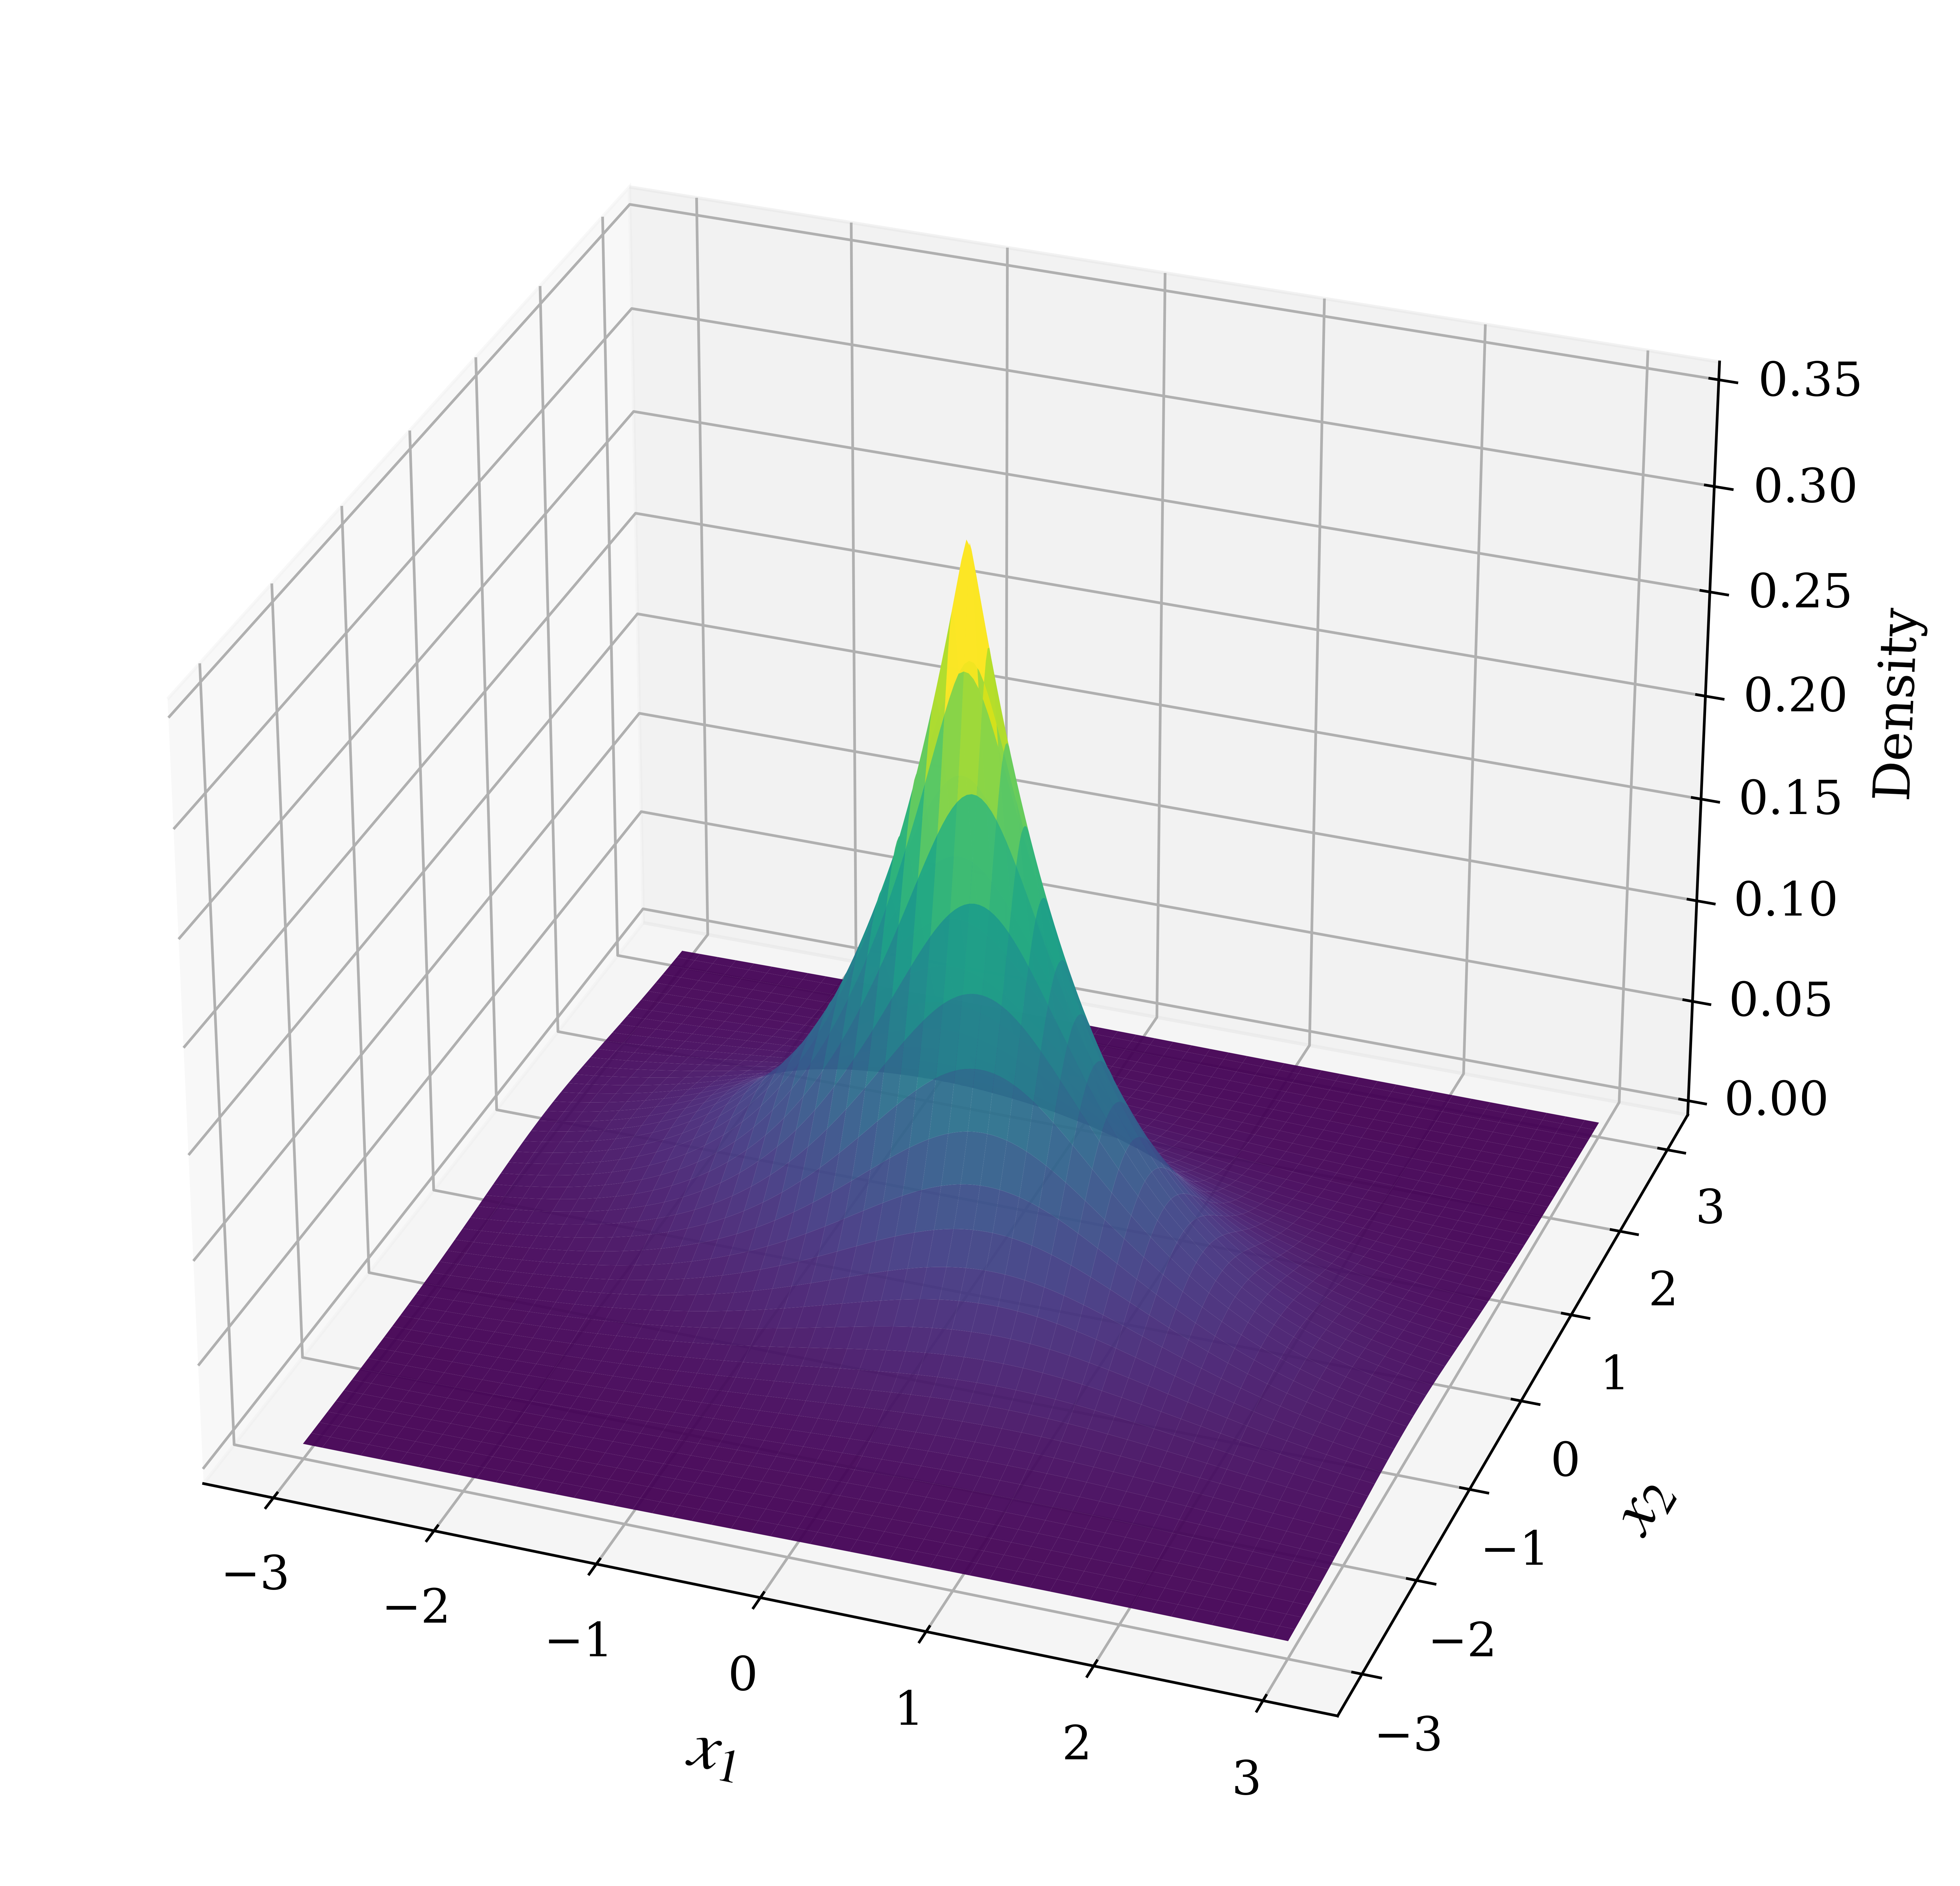
\includegraphics[width=0.5\linewidth]{figures/plot5.png}
    }
    \subfigure[$\;$ $\bmu = (0, 0)^\top$, $\bSi = (2, -0.5; -0.5, 1)$ and $\la = 1$;]
    {
        \centering
        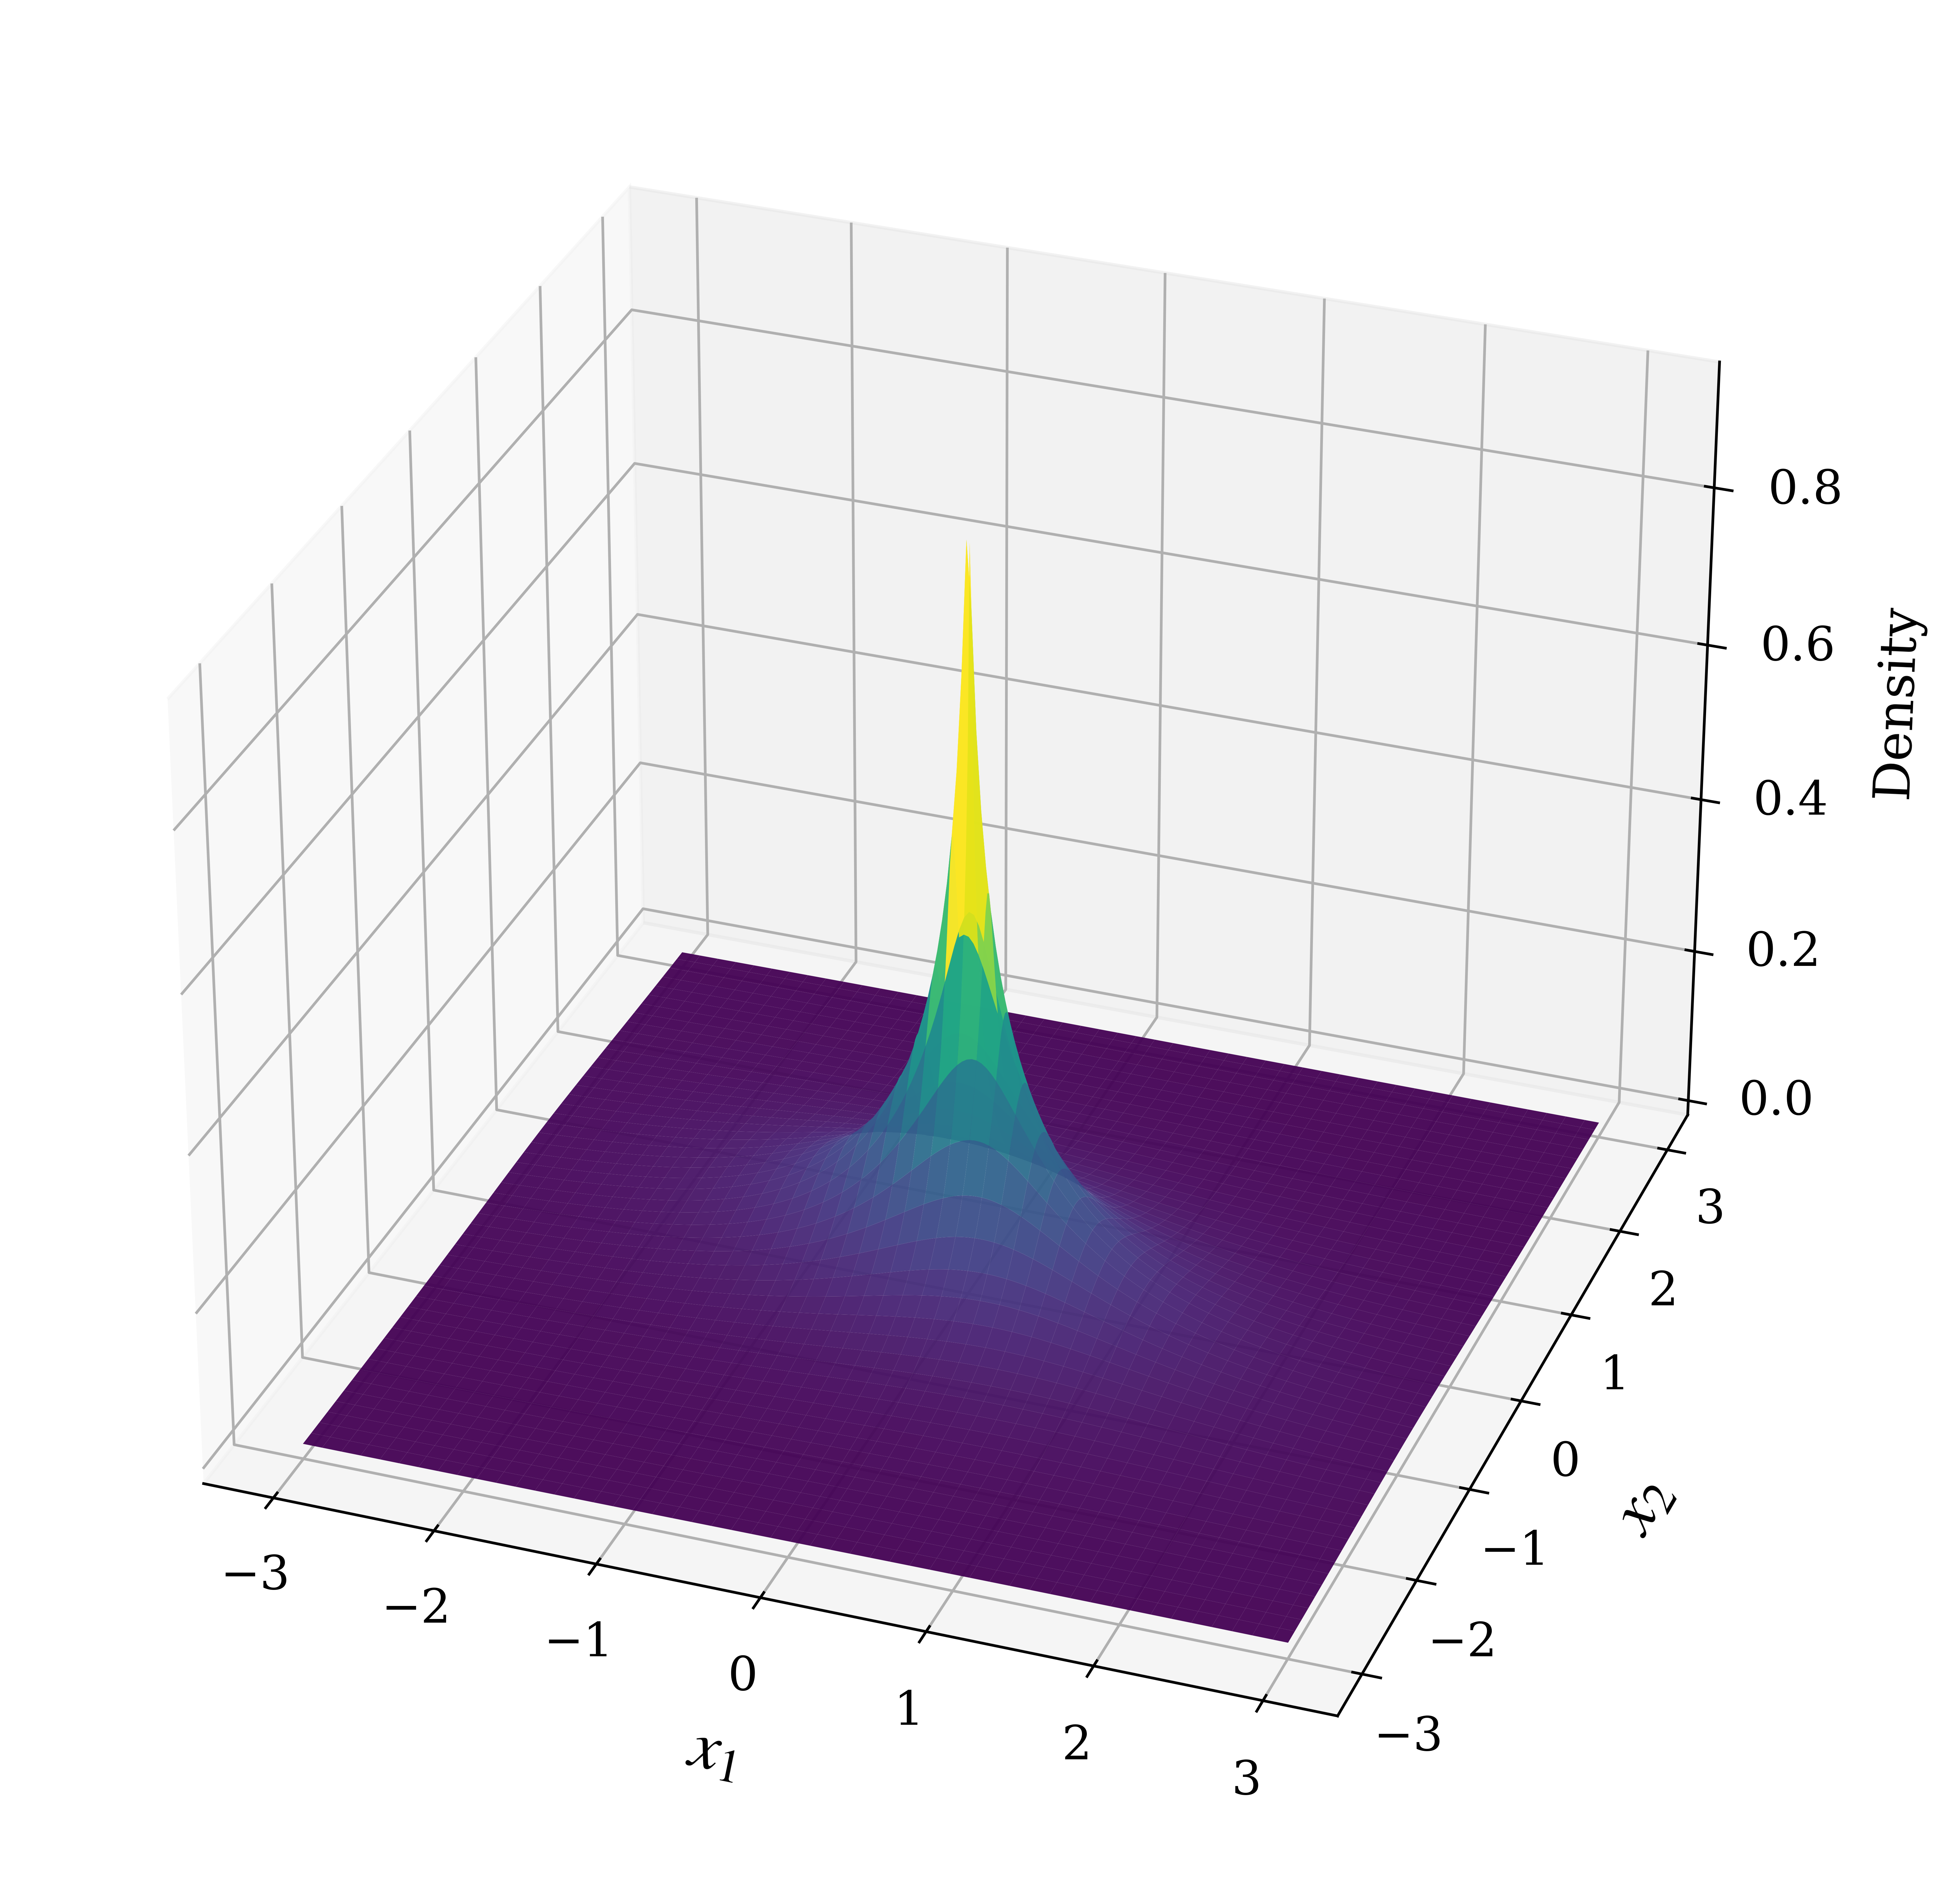
\includegraphics[width=0.5\linewidth]{figures/plot6.png}
    }
    \subfigure[$\;$ $\bmu = (0, 0)^\top$, $\bSi = (2, -0.5; -0.5, 1)$ and $\la = 2$;]
    {
        \centering
        
\includegraphics[width=0.5\linewidth]{figures/plot7.png}
    }
    \subfigure[$\;$ $\bmu = (0, 0)^\top$, $\bSi = (2, 0.5; 0.5, 1)$ and $\la = 2$.]
    {
        \centering
        
\includegraphics[width=0.5\linewidth]{figures/plot8.png}
    }
    \caption{$\;$ Density of $\IGaN$ distribution with various parameter combinations.}
    \label{zyf.four.S.fig2}
\end{figure}
We easily compute the expectation, variance and kurtosis as
\begin{eqnarray*}
    E(\ibX) = \bmu, \quad \Var(\ibX) = \bSi \qand \Kurt(X_j) = \frac{3}{\la}, \quad j = 1, \dots, d.
\end{eqnarray*}
\begin{remark}{\rm \textbf{(Generalized Type I multivariate Laplace distribution).} By observing the SR of Type I multivariate Laplace distribution
$$
    \ibX_L \sd \bmu_L + \frac{\ibZ_L}{\sqrt{\IGamma(1, 1/2)}},
$$
where $\ibZ_L \sim N_d(\0, \bSi_L)$. We found that $\IGaN$ is actually an generalized three--parameter form with $\bmu = \bmu_t$, $\bSi = 2\bSi_t$ and $\la = 1$. Therefore, in \S\ref{zyf.four.S.sec:IGaN}, we will study the statistical inference and construct the mean regression model for IGa-N$_d$ (i.e., three--parameter Type I multivariate Laplace) distribution. \hfill $\|$
}\end{remark}

\subsubsection{Mean regression model and MLEs computation for $\IGaN$}\label{zyf.four.S.sec:IGaN}      % Section S1.2.2

Suppose that $\{\ibX_i\}_{i=1}^n \ind \mbox{IGa-N}_d(\bmu_i, \bSi, \la)$ and $\Y{obs} = \{\ibx_i, \ibzi\}_{i=1}^n$ denote the observed data, we consider the following mean regression model
$$
    E(\ibX_i | \ibzi) = \bmu_i = \bB^\top \ibzi, \quad i = 1, \dots, n, 
$$
where $\ibzi = (z_{i1}, \dots, z_{iq})^\top$ is a $q$-dimensional vector of covariates for the $i$-th subject, the matrix of regression coefficients
\begin{eqnarray*}
    \bB = \left(
    \begin{array}{cccc}
        \be_{11} & \be_{12} & \cdots & \be_{1d} \\ 
        \be_{21} & \be_{22} & \cdots & \be_{2d} \\ 
        \vdots   & \vdots   & \ddots & \vdots   \\
        \be_{q1} & \be_{q2} & \cdots & \be_{qd}
    \end{array}
    \right),
\end{eqnarray*}
with $q \times d + d(d + 1) / 2 + 1 \le n$. Let $\bga = \{ \bB, \bSi, \bla\}$ be the parameter vector, the log-likelihood function of $\bga$ is
\begin{eqnarray*}
    \ell_2(\bga | \Y{obs}) &\sr{\rm (\ref{zyf.four.S1.3})}& -\frac{nd}{2} \log(2\pi) - \frac{n}{2} \log|\bSi| + n\la\log\la - n \log\Ga(\la) \\ [2mm]
    && +\; \sum_{i=1}^n \log \int_0^\infty h_2(\tau | \ibx_i, \ibzi, \bga) \rd \tau,
\end{eqnarray*}
where 
$$
    h_2(\tau | \ibx_i, \ibzi, \bga) \teq \tau^{\frac{d}{2} - \la - 1} \exp\left\{-\frac{1}{2}\left[\left(\ibx - \bB^\top \ibzi\right)^\top \bSi^{-1} \left(\ibx - \bB^\top \ibzi\right) \tau + \frac{2\la}{\tau} \right]\right\}.
$$
To calculate the MLEs of $\bga$, we utilize the N-EM algorithm. By computing the ndf
\begin{eqnarray*}
    g_2(\tau | \ibx_i, \ibzi, \bga) &\teq& \frac{h_2(\tau | \ibx_i, \ibzi, \bga)}{\int_0^\infty h_2(s | \ibx_i, \ibzi, \bga) \rd s} \\ [2mm]
    &=& \GIGau\left( \tau \;\bigg| \left(\ibx_i - \bB^\top\ibzi\right)^\top \bSi^{-1} \left(\ibx_i - \bB^\top \ibzi\right),\; 2\la,\; \frac{d}{2} - \la \right),
\end{eqnarray*}
we construct the surrogate function 
\begin{eqnarray*}
    Q_2(\bga | \bgat) &=& \ct{2} - \frac{n}{2} \log|\bSi| - \frac{1}{2} \sum_{i=1}^n \at{i,2} \left(\ibx_i - \bB^\top \ibzi \right)^\top \bSi^{-1} \left(\ibx_i - \bB^\top \ibzi \right) \\ [2mm]
    && +\; n \left[ \left(\Bbt{2} + \Bdt{2}\right)\la + \la\log\la - \log\Ga(\la) \right],
\end{eqnarray*}
with constant $\ct{2}$ free from $\bga$ and for $i = 1, \dots, n$, 
\begin{eqnarray*}
    && \at{i,2} = \int_0^\infty \tau \cdot g_2(\tau | \ibx_i, \ibzi, \bgat) \rd \tau, \hspace{1cm} \Bat{2} \teq \frac{1}{n} \sum_{i=1}^{n} \at{i,2}, \\ [2mm]
    && \bt{i,2} = \int_0^\infty \frac{1}{\tau} \cdot g_2(\tau | \ibx_i, \ibzi, \bgat) \rd \tau, \hspace{1cm} \Bbt{2} \teq \frac{1}{n} \sum_{i=1}^{n} \bt{i,2}, \\ [2mm]
    && \dt{i,2} = \int_0^\infty \log\tau \cdot g_2(\tau | \ibx_i, \ibzi, \bgat) \rd \tau, \quad \Bdt{2} \teq \frac{1}{n} \sum_{i=1}^{n} \dt{i,2}.
\end{eqnarray*}
By maximizing $Q_2(\bga | \bgat)$ respect to $\bga$, we obtain the $(t+1)$-th approximation of $\hbga$ as
\begin{eqnarray}
    \bBtI &=& \left[ \sum_{i=1}^n \at{i,2} \ibzi \ibziT \right]^{-1} \left[ \sum_{i=1}^n \at{i,2} \ibzi \ibx_i^\top \right] = \left(\bZ^\top \At{2} \bZ\right)^{-1} \left(\bZ^\top \At{2} \bX\right), \non \\ [2mm]
    \bSitI &=& \frac{1}{n} \sum_{i=1}^n \at{i,2} \left( \ibx_i - \bB^{(t+1)\top} \ibzi\right) \left( \ibx_i - \bB^{(t+1)\top}\ibzi \right)^\top \non \\ [2mm]
    &=& \frac{1}{n}\left(\bX - \bZ \bBtI \right)^\top \At{2} \left(\bX - \bZ \bBtI \right), \non \\ [2mm]
    \latI &=& \sol\left\{ 1 - \Bbt{2} - \Bdt{2} + \log\la - \psi(\la) = 0, \quad \la > 0 \right\}, \label{zyf.four.S1.4}
\end{eqnarray}
where $\bZ = (\ibz_{(1)}, \dots, \ibz_{(n)})^\top$, $\At{2} = \diag(\at{1,2}, \dots, \at{n,2})$, $\bX = (\ibx_1, \dots, \ibx_n)^\top$ and the solution in (\ref{zyf.four.S1.4}) can be solved by the US algorithm as shown in \S\ref{zyf.four.S.sec:US2}.

\subsection{The inverse Gaussian mixture of multivariate normal distribution}       % Section S1.3

It is easy to show that if $Y \sim \IGaussian(\mu, \la)$ (\cite{CF1988}) with pdf
$$
    \IGaussian(y|\mu, \la) = \sqrt{\frac{\la}{2\pi}} y^{-\frac{3}{2}} \exp\left[ -\frac{\la (y - \mu)^2}{2\mu^2 y} \right], \quad y > 0, \; \mu > 0, \; \la > 0,
$$
then we have $cY \sim \IGaussian(c\mu, c\la)$ for any constant $c > 0$. Let $Z^* \sim N_d(\0, \bSi^*)$, $\tau^* \sim \IGaussian(\mu^*, \la^*)$ and $Z^* \inde \tau^*$. If we define $\ibX \sd \bmu + Z^* / \sqrt{\tau^*}$, then
\begin{eqnarray*}
    \ibX &\sd& \bmu + \frac{N_d(\0, \bSi^*)}{\IGaussian(\mu^*, \la^*)} = \bmu + \frac{N_d(\0, \bSi^*)}{\sqrt{\la^* / \la \cdot \IGaussian(\la / (\la - 1), \la)}} \\ [2mm]
    &=& \bmu + \frac{N_d(\0, \frac{\la}{\la^*} \bSi^*)}{\sqrt{\IGaussian(\la / (\la - 1), \la)}} = \bmu + \frac{N_d(\0, \bSi)}{\sqrt{\IGaussian(\la / (\la - 1), \la)}},
\end{eqnarray*}
where $\bSi = \la \bSi^* / \la^*$ and $\tau \sim \IGaussian(\la / (\la - 1), \la)$ with $\la \teq (\mu^* + \la^*) / \mu^*$ and $E(\tau^{-1}) = 1$ for any $\la > 1$, which can motivate the following definition.

\subsubsection{Definition and basic properties of the IGau-N$_d$ distribution}        % Section S1.3.1

\begin{definition}{\rm \textbf{(IGau-N$_d$ distribution).} Suppose that $\tau \sim \IGaussian(\la / (\la - 1), \la)$ with $\la > 1$ and the SR:
$$
    \ibX \sd \bmu + \frac{\ibZ}{\sqrt{\tau}}, 
$$
where $\bmu = (\mu_1, \dots, \mu_d)^\top \in \bbR^d$ is the location parameter, $\ibZ = (Z_1, \dots, Z_d)^\top \sim N_d(\0, \bSi)$ with scale matrix $\bSi = (\sigma_{ij})_{d\times d}$ and $\ibZ \inde \tau$, then the \trv $\ibX = (X_1, \dots, X_d)^\top$ is said to follow the IGau-N$_d$ distribution, denoted by $\ibX \sim \IGauN$ or IGau-N$_d(\bth)$, where $\bth = \{\bmu, \bSi, \la\}$ is the parameter vector. \hfill $\|$
}\end{definition}

Set $f_\tau(\tau|\bla) = \IGaussian(\tau|\la / (\la - 1), \la)$, we obtain the pdf of $\ibX \sim \IGauN$ as
\begin{eqnarray}
    \mbox{IGau-N}_d(\ibx|\bth) &=& \frac{\e^{\la - 1}\sqrt{\la}}{(2\pi)^\frac{d + 1}{2} |\bSi|^\frac{1}{2}} \int_0^\infty h_{3*}(\tau | \ibx, \bth) \rd \tau \label{zyf.four.S1.5} \\ [2mm]
    &=& \frac{\e^{\la - 1}\sqrt{\la}}{2^\frac{d - 1}{2} \pi^\frac{d + 1}{2} |\bSi|^\frac{1}{2}} \cdot K_\frac{d - 1}{2}\left( \sqrt{(\ibx - \bmu)^\top \bSi^{-1} (\ibx - \bmu) \la + (\la - 1)^2} \right) \non \\ [2mm] 
    && \times\; \left[ \frac{(\ibx - \bmu)^\top \bSi^{-1} (\ibx - \bmu)}{\la} + \left( \frac{\la - 1}{\la} \right)^2\right]^{-\frac{d-1}{4}}, \non
\end{eqnarray}
where 
\begin{eqnarray*}
    h_{3*}(\tau | \ibx, \bth) = \tau^\frac{d - 3}{2} \exp\left\{-\frac{1}{2}\left[\left((\ibx - \bmu)^\top \bSi^{-1} (\ibx - \bmu) + \frac{(\la - 1)^2}{\la} \right) \tau + \frac{\la}{\tau} \right]\right\}.
\end{eqnarray*}
\begin{figure}[H]
    \subfigure[$\;$ $\bmu = (0, 0)^\top$, $\bSi = (1, -0.75; -0.75, 1)$ and $\la = 1.5$;]
    {
        \centering
        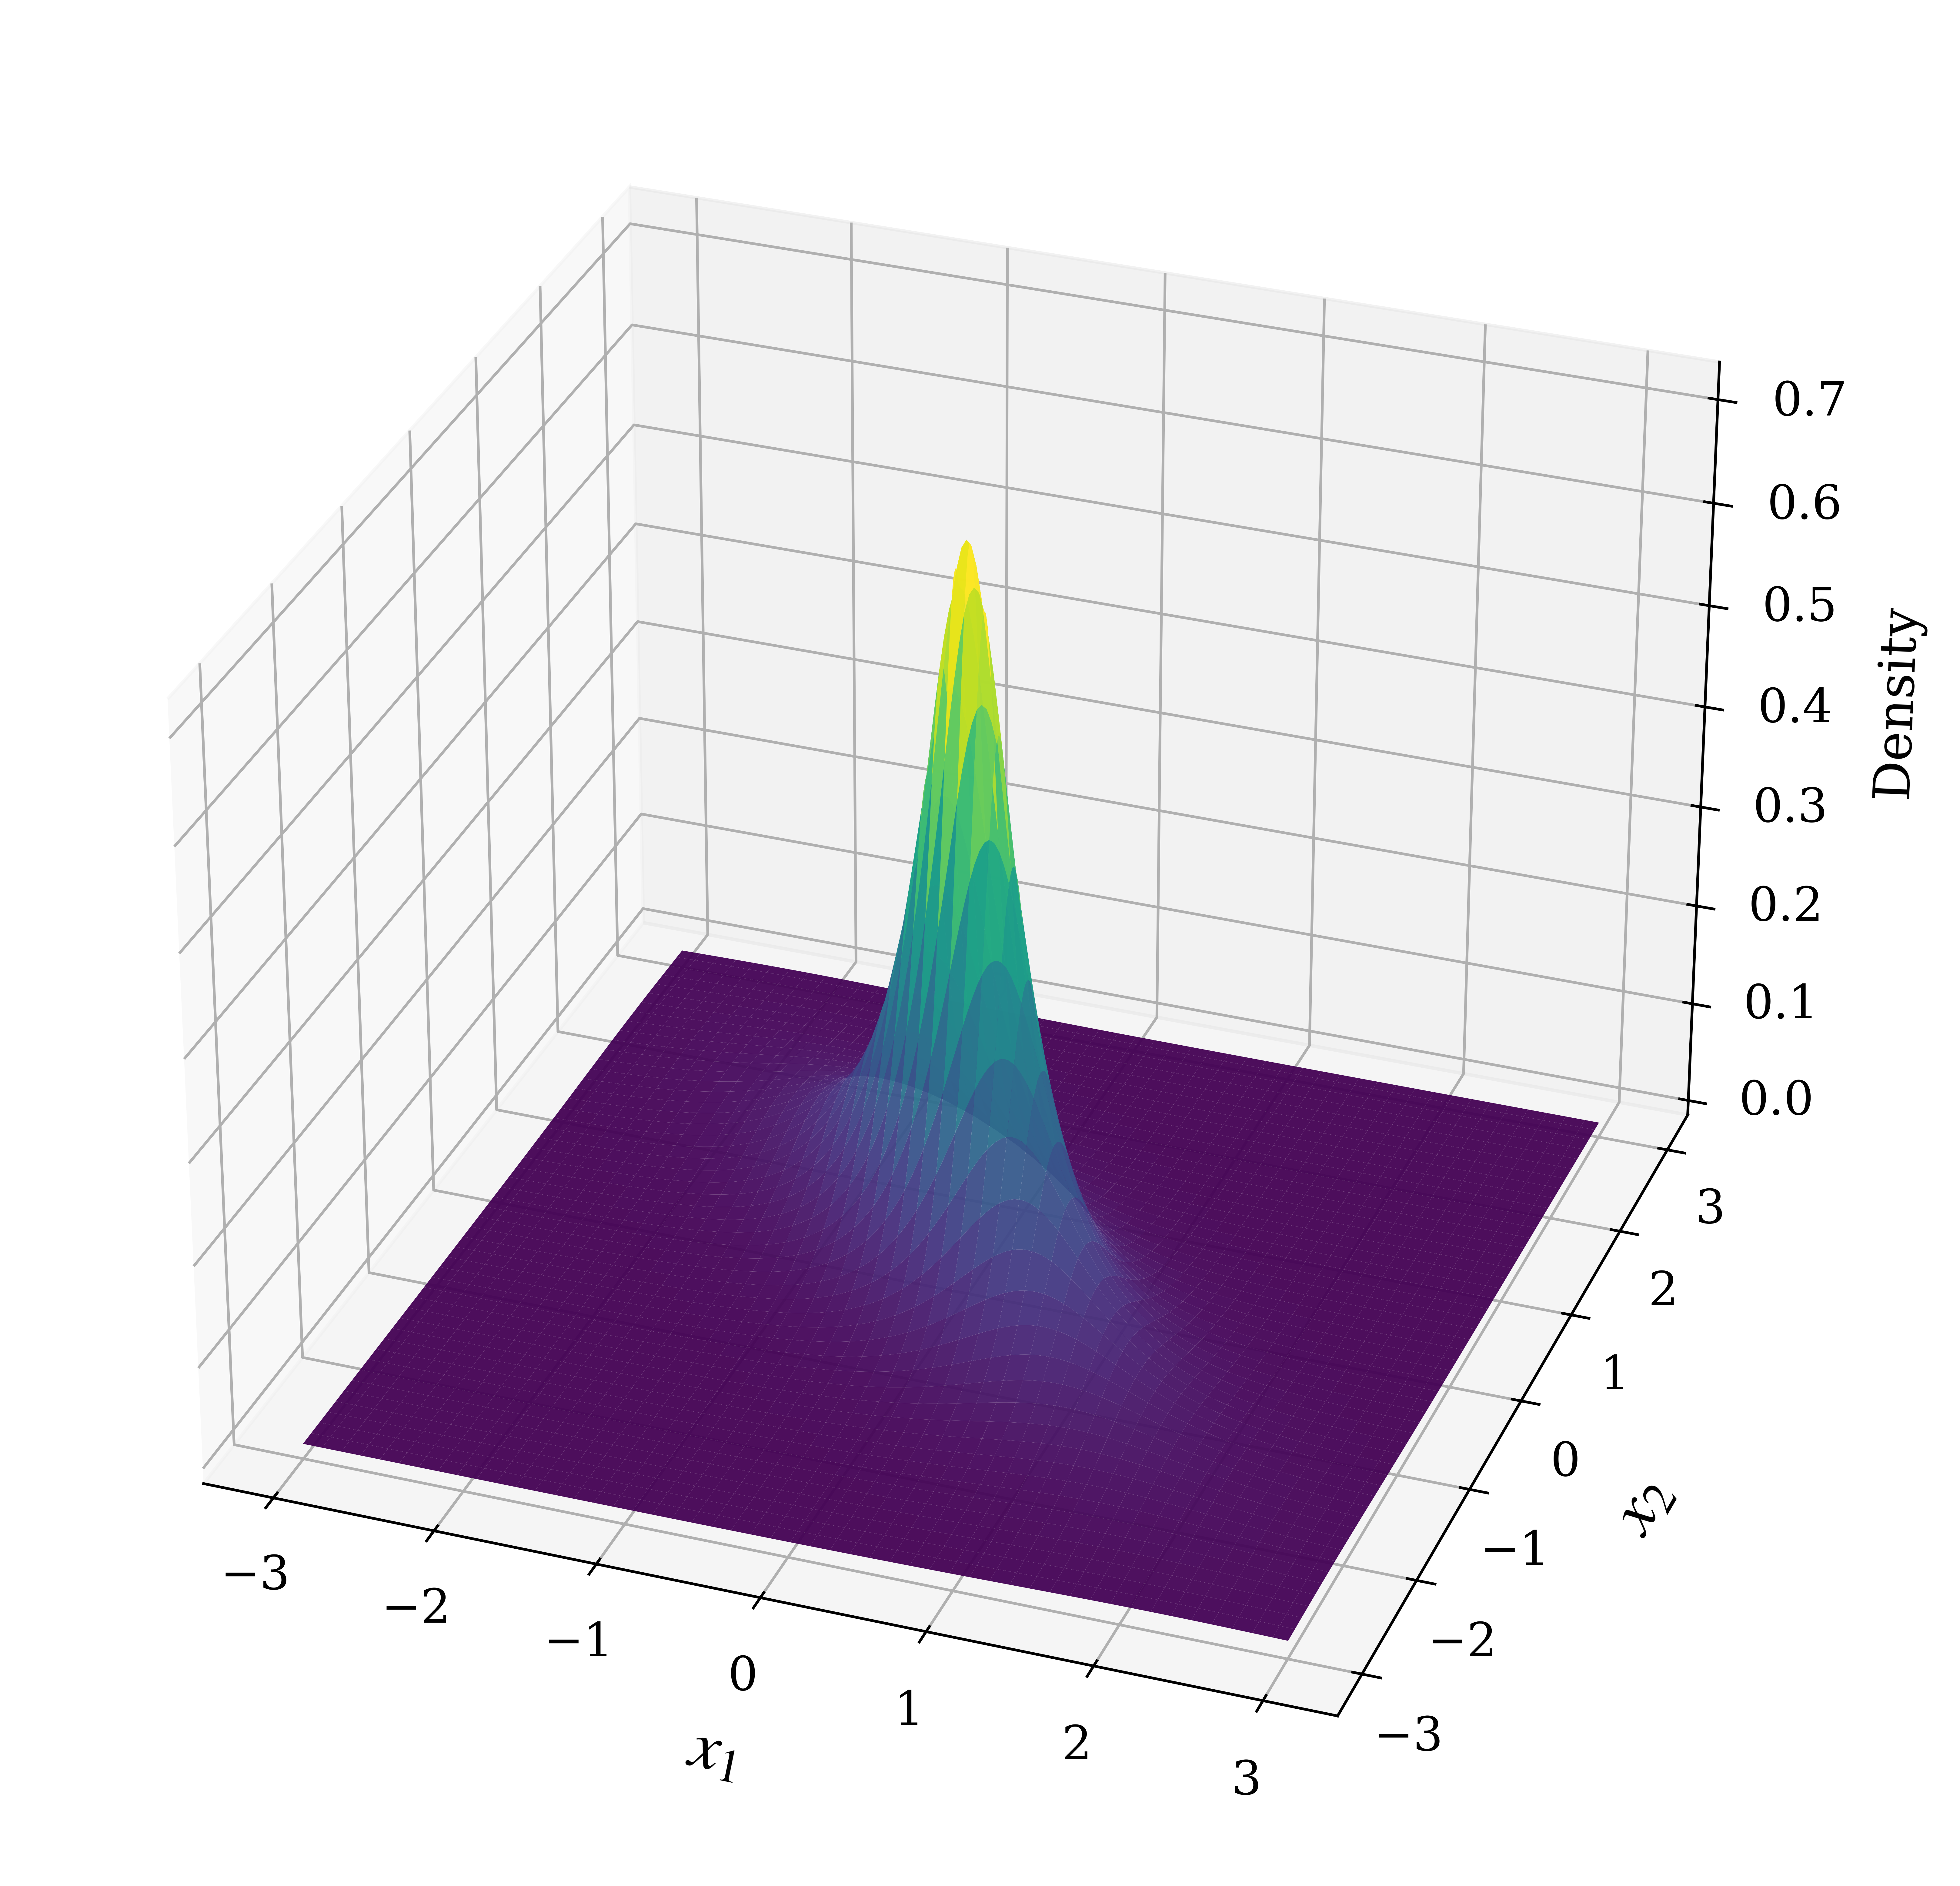
\includegraphics[width=0.5\linewidth]{figures/plot9.png}
    }
    \subfigure[$\;$ $\bmu = (0, 0)^\top$, $\bSi = (1, -0.75; -0.75, 1)$ and $\la = 3$;]
    {
        \centering
        
\includegraphics[width=0.5\linewidth]{figures/plot10.png}
    }
    \subfigure[$\;$ $\bmu = (0, 0)^\top$, $\bSi = (1, 0.5; 0.5, 1)$ and $\la = 1.5$;]
    {
        \centering
        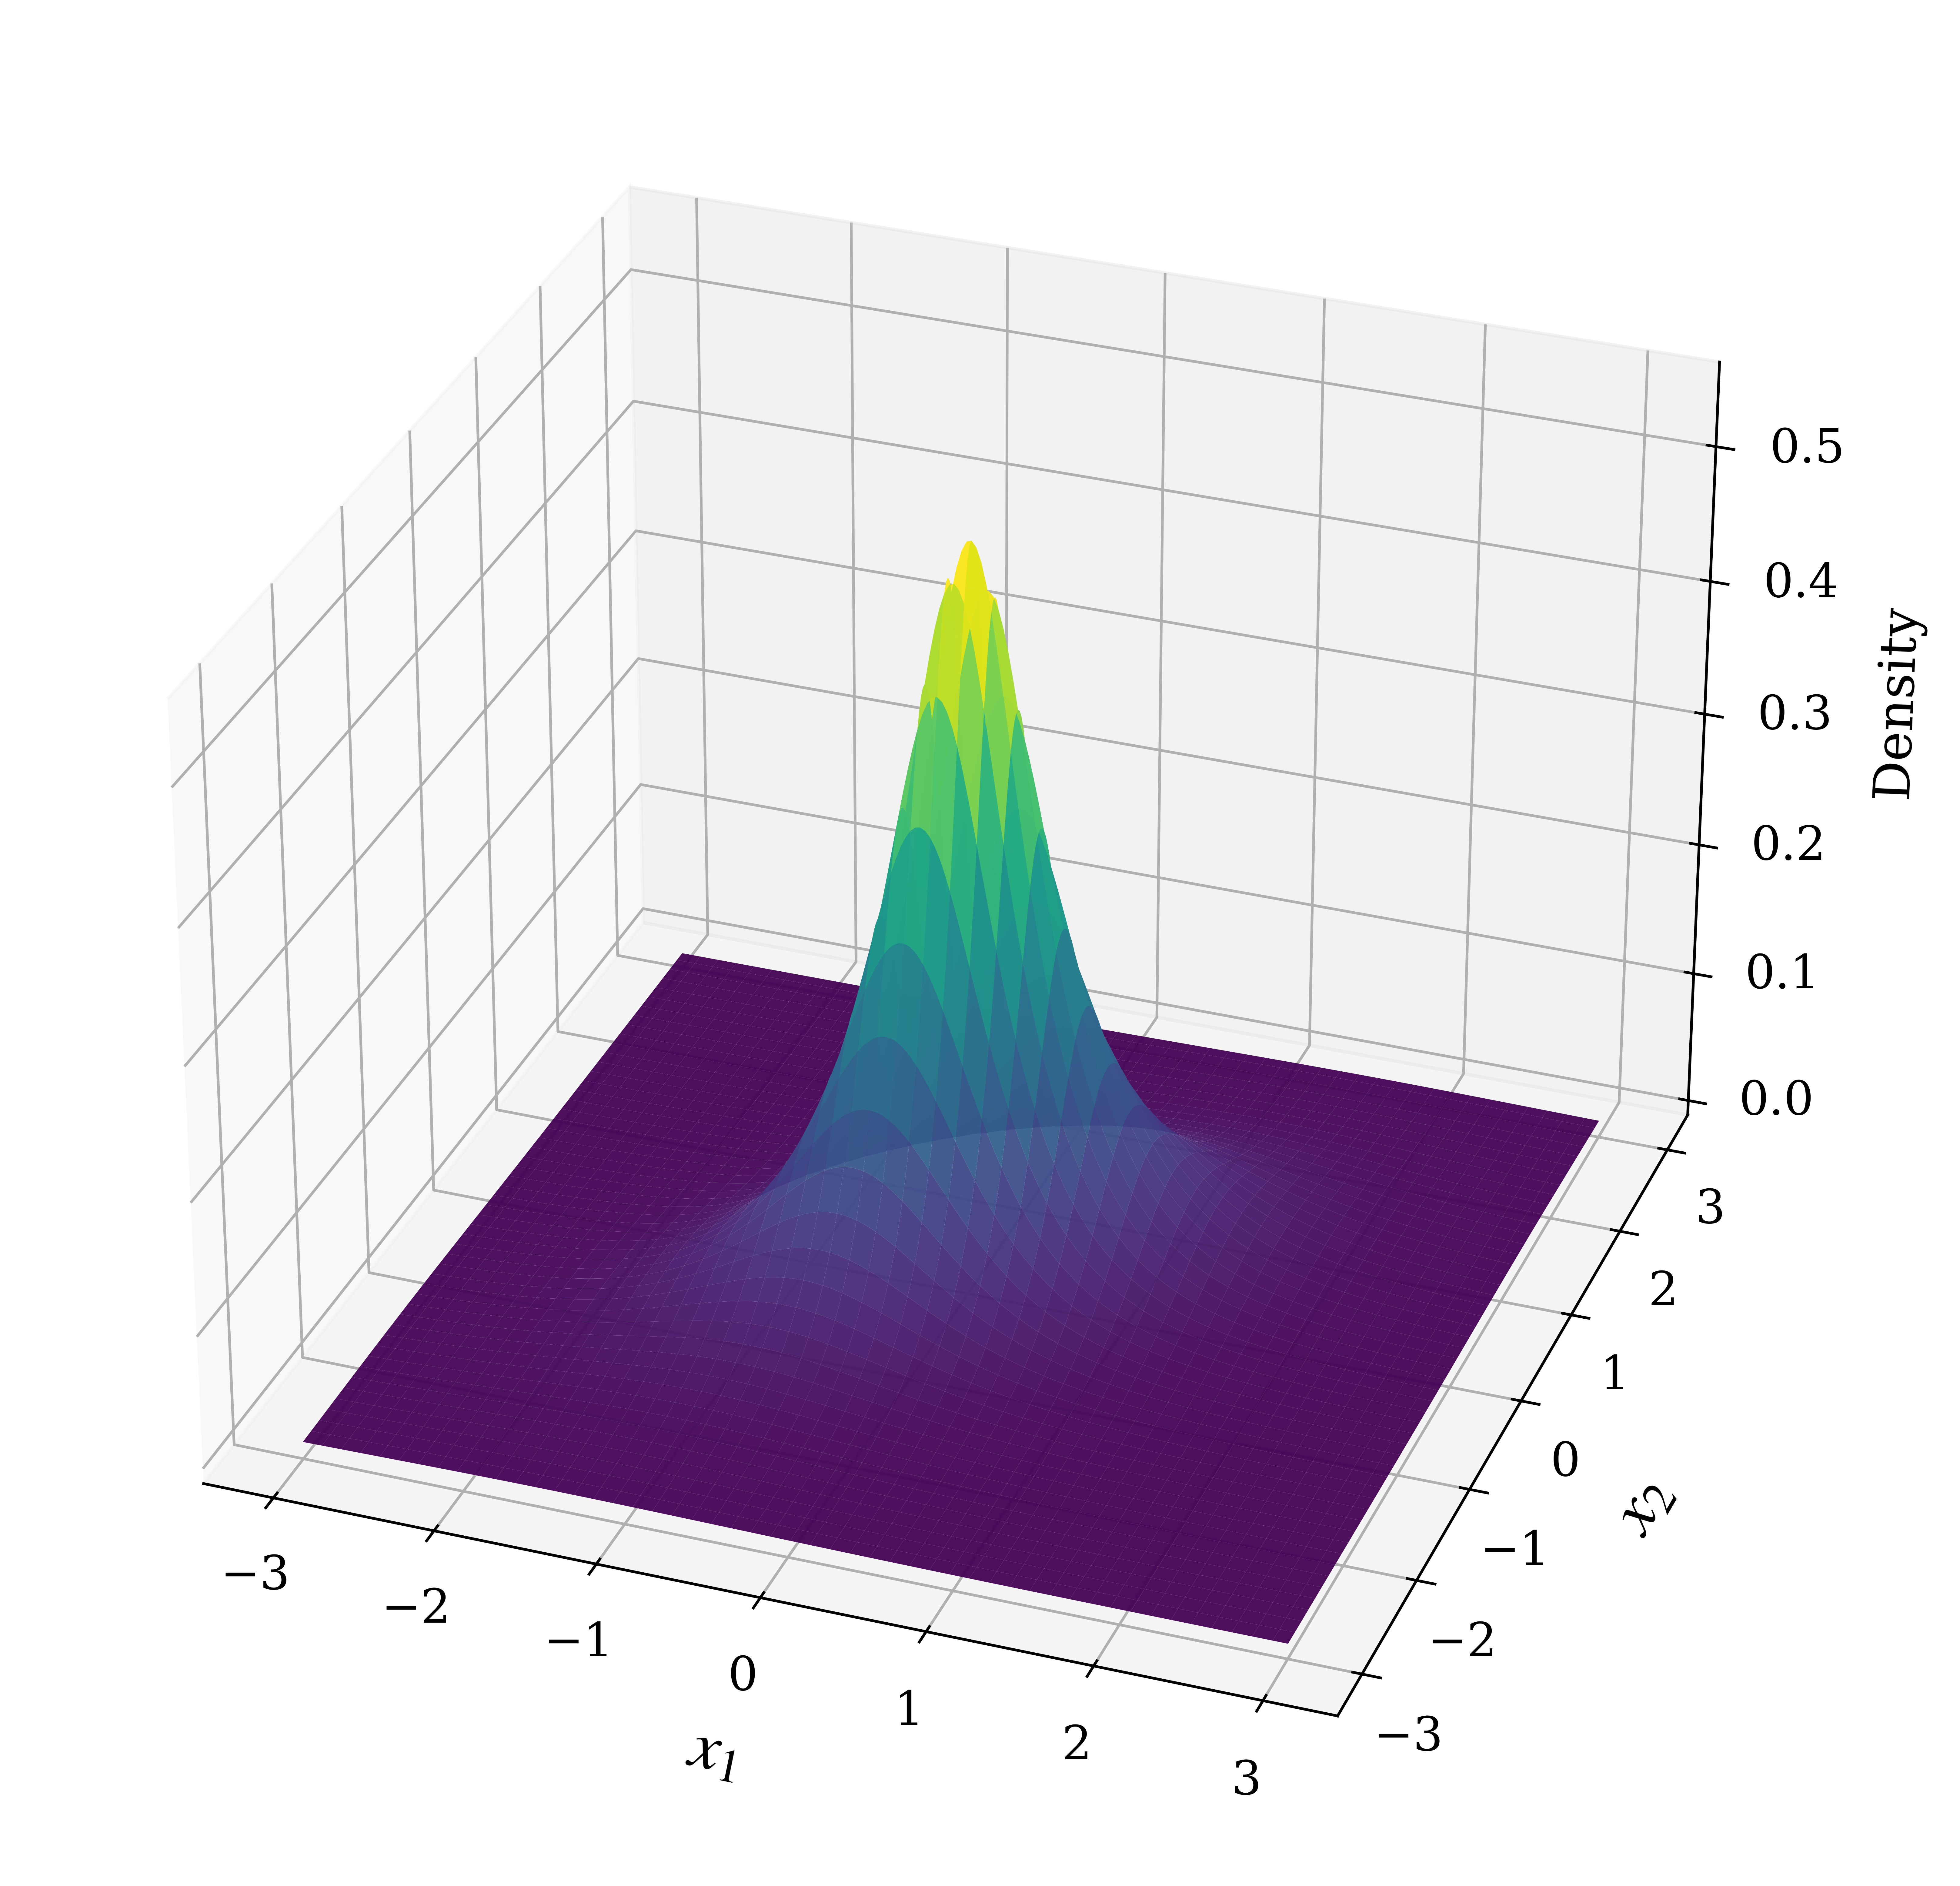
\includegraphics[width=0.5\linewidth]{figures/plot11.png}
    }
    \subfigure[$\;$ $\bmu = (0, 0)^\top$, $\bSi = (1, 0.5; 0.5, 1)$ and $\la = 3$.]
    {
        \centering
        
\includegraphics[width=0.5\linewidth]{figures/plot12.png}
    }
    \caption{$\;$ Density of $\IGauN$ distribution with various parameter combinations.}
    \label{zyf.four.S.fig3}
\end{figure}
We easily compute the expectation, variance and kurtosis as
\begin{eqnarray*}
    E(\ibX) = \bmu, \quad \Var(\ibX) = \bSi \qand \Kurt(X_j) = \frac{3(\la + 1)}{\la^2}, \quad j = 1, \dots, d.
\end{eqnarray*}

\subsubsection{Mean regression model and MLEs computation for $\IGauN$}       % Section S1.3.2

Suppose that $\{\ibX_i\}_{i=1}^n \ind \mbox{IGau-N}_d(\bmu_i, \bSi, \la)$ and $\Y{obs} = \{\ibx_i, \ibzi\}_{i=1}^n$ denote the observed data, we consider the following mean regression model
$$
    E(\ibX_i | \ibzi) = \bmu_i = \bB^\top \ibzi, \quad i = 1, \dots, n, 
$$
where $\ibzi = (z_{i1}, \dots, z_{iq})^\top$ is a $q$-dimensional vector of covariates for the $i$-th subject, the matrix of regression coefficients
\begin{eqnarray*}
    \bB = \left(
    \begin{array}{cccc}
        \be_{11} & \be_{12} & \cdots & \be_{1d} \\ 
        \be_{21} & \be_{22} & \cdots & \be_{2d} \\ 
        \vdots   & \vdots   & \ddots & \vdots   \\
        \be_{q1} & \be_{q2} & \cdots & \be_{qd}
    \end{array}
    \right),
\end{eqnarray*}
with $q \times d + d(d + 1) / 2 + 1 \le n$. Let $\bga = \{ \bB, \bSi, \bla\}$ be the parameter vector, the log-likelihood function of $\bga$ is
\begin{eqnarray*}
    \ell_3(\bga | \Y{obs}) &\sr{\rm (\ref{zyf.four.S1.5})}& -\frac{n(d + 1)}{2} \log(2\pi) - \frac{n}{2} \log|\bSi| + n(\la - 1) + \frac{n}{2} \log\la \\ [2mm]
    && +\; \sum_{i=1}^n \log \int_0^\infty h_3(\tau | \ibx_i, \ibzi, \bga) \rd \tau,
\end{eqnarray*}
where 
$$
    h_3(\tau | \ibx_i, \ibzi, \bga) \teq \tau^\frac{d - 3}{2} \exp\left\{-\frac{1}{2}\left[\left(\left(\ibx - \bB^\top \ibzi\right)^\top \bSi^{-1} \left(\ibx - \bB^\top \ibzi\right) + \frac{(\la - 1)^2}{\la} \right) \tau + \frac{\la}{\tau} \right]\right\}.
$$
To calculate the MLEs of $\bga$, we utilize the N-EM algorithm. By computing the ndf
\begin{eqnarray*}
    g_3(\tau | \ibx_i, \ibzi, \bga) &\teq& \frac{h_3(\tau | \ibx_i, \ibzi, \bga)}{\int_0^\infty h_3(s | \ibx_i, \ibzi, \bga) \rd s} \\ [2mm]
    &=& \GIGau\left( \tau \;\bigg| \left(\ibx_i - \bB^\top\ibzi\right)^\top \bSi^{-1} \left(\ibx_i - \bB^\top \ibzi\right) + \frac{(\la - 1)^2}{\la},\; \la,\; \frac{d - 1}{2}\right),
\end{eqnarray*}
we construct the surrogate function 
\begin{eqnarray*}
    Q_3(\bga | \bgat) &=& \ct{3} - \frac{n}{2} \log|\bSi| - \frac{1}{2} \sum_{i=1}^n \at{i,3} \left(\ibx_i - \bB^\top \ibzi \right)^\top \bSi^{-1} \left(\ibx_i - \bB^\top \ibzi \right) \\ [2mm]
    && +\; \frac{n}{2} \left[ \left(2 - \Bat{3} - \Bbt{3}\right) \la - \frac{\Bat{3}}{\la} + \log\la \right],
\end{eqnarray*}
with constant $\ct{3}$ free from $\bga$ and for $i = 1, \dots, n$, 
\begin{eqnarray*}
    && \at{i,3} = \int_0^\infty \tau \cdot g_3(\tau | \ibx_i, \ibzi, \bgat) \rd \tau, \quad \Bat{3} \teq \frac{1}{n} \sum_{i=1}^{n} \at{i,3}, \\ [2mm]
    && \bt{i,3} = \int_0^\infty \frac{1}{\tau} \cdot g_3(\tau | \ibx_i, \ibzi, \bgat) \rd \tau, \quad \Bbt{3} \teq \frac{1}{n} \sum_{i=1}^{n} \bt{i,3}.
\end{eqnarray*}
By maximizing $Q_3(\bga | \bgat)$ respect to $\bga$, we obtain the $(t+1)$-th approximation of $\hbga$ as
\begin{eqnarray*}
    \bBtI &=& \left[ \sum_{i=1}^n \at{i,3} \ibzi \ibziT \right]^{-1} \left[ \sum_{i=1}^n \at{i,3} \ibzi \ibx_i^\top \right] = \left(\bZ^\top \At{3} \bZ\right)^{-1} \left(\bZ^\top \At{3} \bX\right), \\ [2mm]
    \bSitI &=& \frac{1}{n} \sum_{i=1}^n \at{i,3} \left( \ibx_i - \bB^{(t+1)\top} \ibzi\right) \left( \ibx_i - \bB^{(t+1)\top}\ibzi \right)^\top \\ [2mm]
    &=& \frac{1}{n}\left(\bX - \bZ \bBtI \right)^\top \At{3} \left(\bX - \bZ \bBtI \right), \\ [2mm]
    \latI &=& \frac{-1 - \sqrt{1 - 4\Bat{3}\left(2 - \Bat{3} - \Bbt{3}\right)}}{2\left(2 - \Bat{3} - \Bbt{3}\right)},
\end{eqnarray*}
where $\bZ = (\ibz_{(1)}, \dots, \ibz_{(n)})^\top$, $\At{3} = \diag(\at{1,3}, \dots, \at{n,3})$ and $\bX = (\ibx_1, \dots, \ibx_n)^\top$.

\subsection{The reciprocal inverse Gaussian mixture of multivariate normal distribution}       % Section S1.4

Suppose that $X \sim \IGaussian(\mu, \la)$ with parameters $\mu, \la > 0$, then $Y = 1 / X$ is said to follow the \textit{reciprocal inverse Gaussian} (RIGau) distribution, denoted by $Y \sim \RIGau(\mu, \la)$ with pdf
$$
    \RIGau(y|\mu, \la) = \sqrt{\frac{\la}{2\pi y}} \exp\left[ -\frac{\la(1 - \mu y)^2}{2\mu^2 y} \right], \quad y > 0,
$$
where $E(Y^{-1}) = \mu$. It is easy to show that if $Y \sim \RIGau(\mu, \la)$, then $cY \sim \RIGau(\mu / c, \la / c)$ for any constant $c > 0$. Let $Z^* \sim N_d(\0, \bSi^*)$, $\tau^* \sim \RIGau(\mu^*, \la^*)$ and $Z^* \inde \tau^*$. If we define $\ibX \sd \bmu + Z^* / \sqrt{\tau^*}$, then
\begin{eqnarray*}
    \ibX &\sd& \bmu + \frac{N_d(\0, \bSi^*)}{\RIGau(\mu^*, \la^*)} = \bmu + \frac{N_d(\0, \bSi^*)}{\sqrt{\RIGau(1, \la^* / \mu^*) / \mu^*}} \\ [2mm]
    &=& \bmu + \frac{N_d(\0, \mu^* \bSi^*)}{\sqrt{\RIGau(1, \la^* / \mu^*)}} = \bmu + \frac{N_d(\0, \bSi)}{\sqrt{\RIGau(1, \la)}},
\end{eqnarray*}
where $\bSi = \mu^* \bSi^*$ and $\tau \sim \RIGau(1, \la)$ with $\la \teq \la^* / \mu^*$ and $E(\tau^{-1}) = 1$, which can motivate the following definition.

\subsubsection{Definition and basic properties of the RIGau-N$_d$ distribution}        % Section S1.4.1

\begin{definition}{\rm \textbf{(RIGau-N$_d$ distribution).} Suppose that $\tau \sim \RIGau(1, \la)$ and the SR:
$$
    \ibX \sd \bmu + \frac{\ibZ}{\sqrt{\tau}}, 
$$
where $\bmu = (\mu_1, \dots, \mu_d)^\top \in \bbR^d$ is the location parameter, $\ibZ = (Z_1, \dots, Z_d)^\top \sim N_d(\0, \bSi)$ with scale matrix $\bSi = (\sigma_{ij})_{d\times d}$ and $\ibZ \inde \tau$, then the \trv $\ibX = (X_1, \dots, X_d)^\top$ is said to follow the RIGau-N$_d$ distribution, denoted by $\ibX \sim \RIGauN$ or RIGau-N$_d(\bth)$, where $\bth = \{\bmu, \bSi, \la\}$ is the parameter vector. \hfill $\|$
}\end{definition}

Set $f_\tau(\tau|\bla) = \RIGau(\tau| 1, \la)$, we obtain the pdf of $\ibX \sim \RIGauN$ as
\begin{eqnarray}
    \mbox{RIGau-N}_d(\ibx|\bth) &=& \frac{\e^\la \sqrt{\la}}{(2\pi)^\frac{d + 1}{2} |\bSi|^\frac{1}{2}} \int_0^\infty h_{4*}(\tau | \ibx, \bth) \rd \tau \label{zyf.four.S1.6} \\ [2mm]
    &=& \frac{\e^\la \sqrt{\la}}{2^\frac{d - 1}{2} \pi^\frac{d + 1}{2} |\bSi|^\frac{1}{2}} \cdot K_\frac{d + 1}{2}\left( \sqrt{\la\left[ (\ibx - \bmu)^\top \bSi^{-1} (\ibx - \bmu) + \la \right]} \right) \non \\ [2mm] 
    && \times\; \left[ \frac{(\ibx - \bmu)^\top \bSi^{-1} (\ibx - \bmu)}{\la} + 1 \right]^{-\frac{d + 1}{4}}, \non
\end{eqnarray}
where 
\begin{eqnarray*}
    h_{4*}(\tau | \ibx, \bth) = \tau^\frac{d - 1}{2} \exp\left\{-\frac{1}{2}\left[\left((\ibx - \bmu)^\top \bSi^{-1} (\ibx - \bmu) + \la \right) \tau + \frac{\la}{\tau} \right]\right\}.
\end{eqnarray*}
We easily compute the expectation, variance and kurtosis as
\begin{eqnarray*}
    E(\ibX) = \bmu, \quad \Var(\ibX) = \bSi \qand \Kurt(X_j) = \frac{3}{\la}, \quad j = 1, \dots, d.
\end{eqnarray*}
\begin{figure}[H]
    \subfigure[$\;$ $\bmu = (0, 0)^\top$, $\bSi = (1, 0; 0, 2)$ and $\la = 0.5$;]
    {
        \centering
        
\includegraphics[width=0.5\linewidth]{figures/plot13.png}
    }
    \subfigure[$\;$ $\bmu = (0, 0)^\top$, $\bSi = (1, 0; 0, 2)$ and $\la = 2$;]
    {
        \centering
        
\includegraphics[width=0.5\linewidth]{figures/plot14.png}
    }
    \subfigure[$\;$ $\bmu = (0, 0)^\top$, $\bSi = (1, 0.5; 0.5, 2)$ and $\la = 0.5$;]
    {
        \centering
        
\includegraphics[width=0.5\linewidth]{figures/plot15.png}
    }
    \subfigure[$\;$ $\bmu = (0, 0)^\top$, $\bSi = (1, 0.5; 0.5, 2)$ and $\la = 2$.]
    {
        \centering
        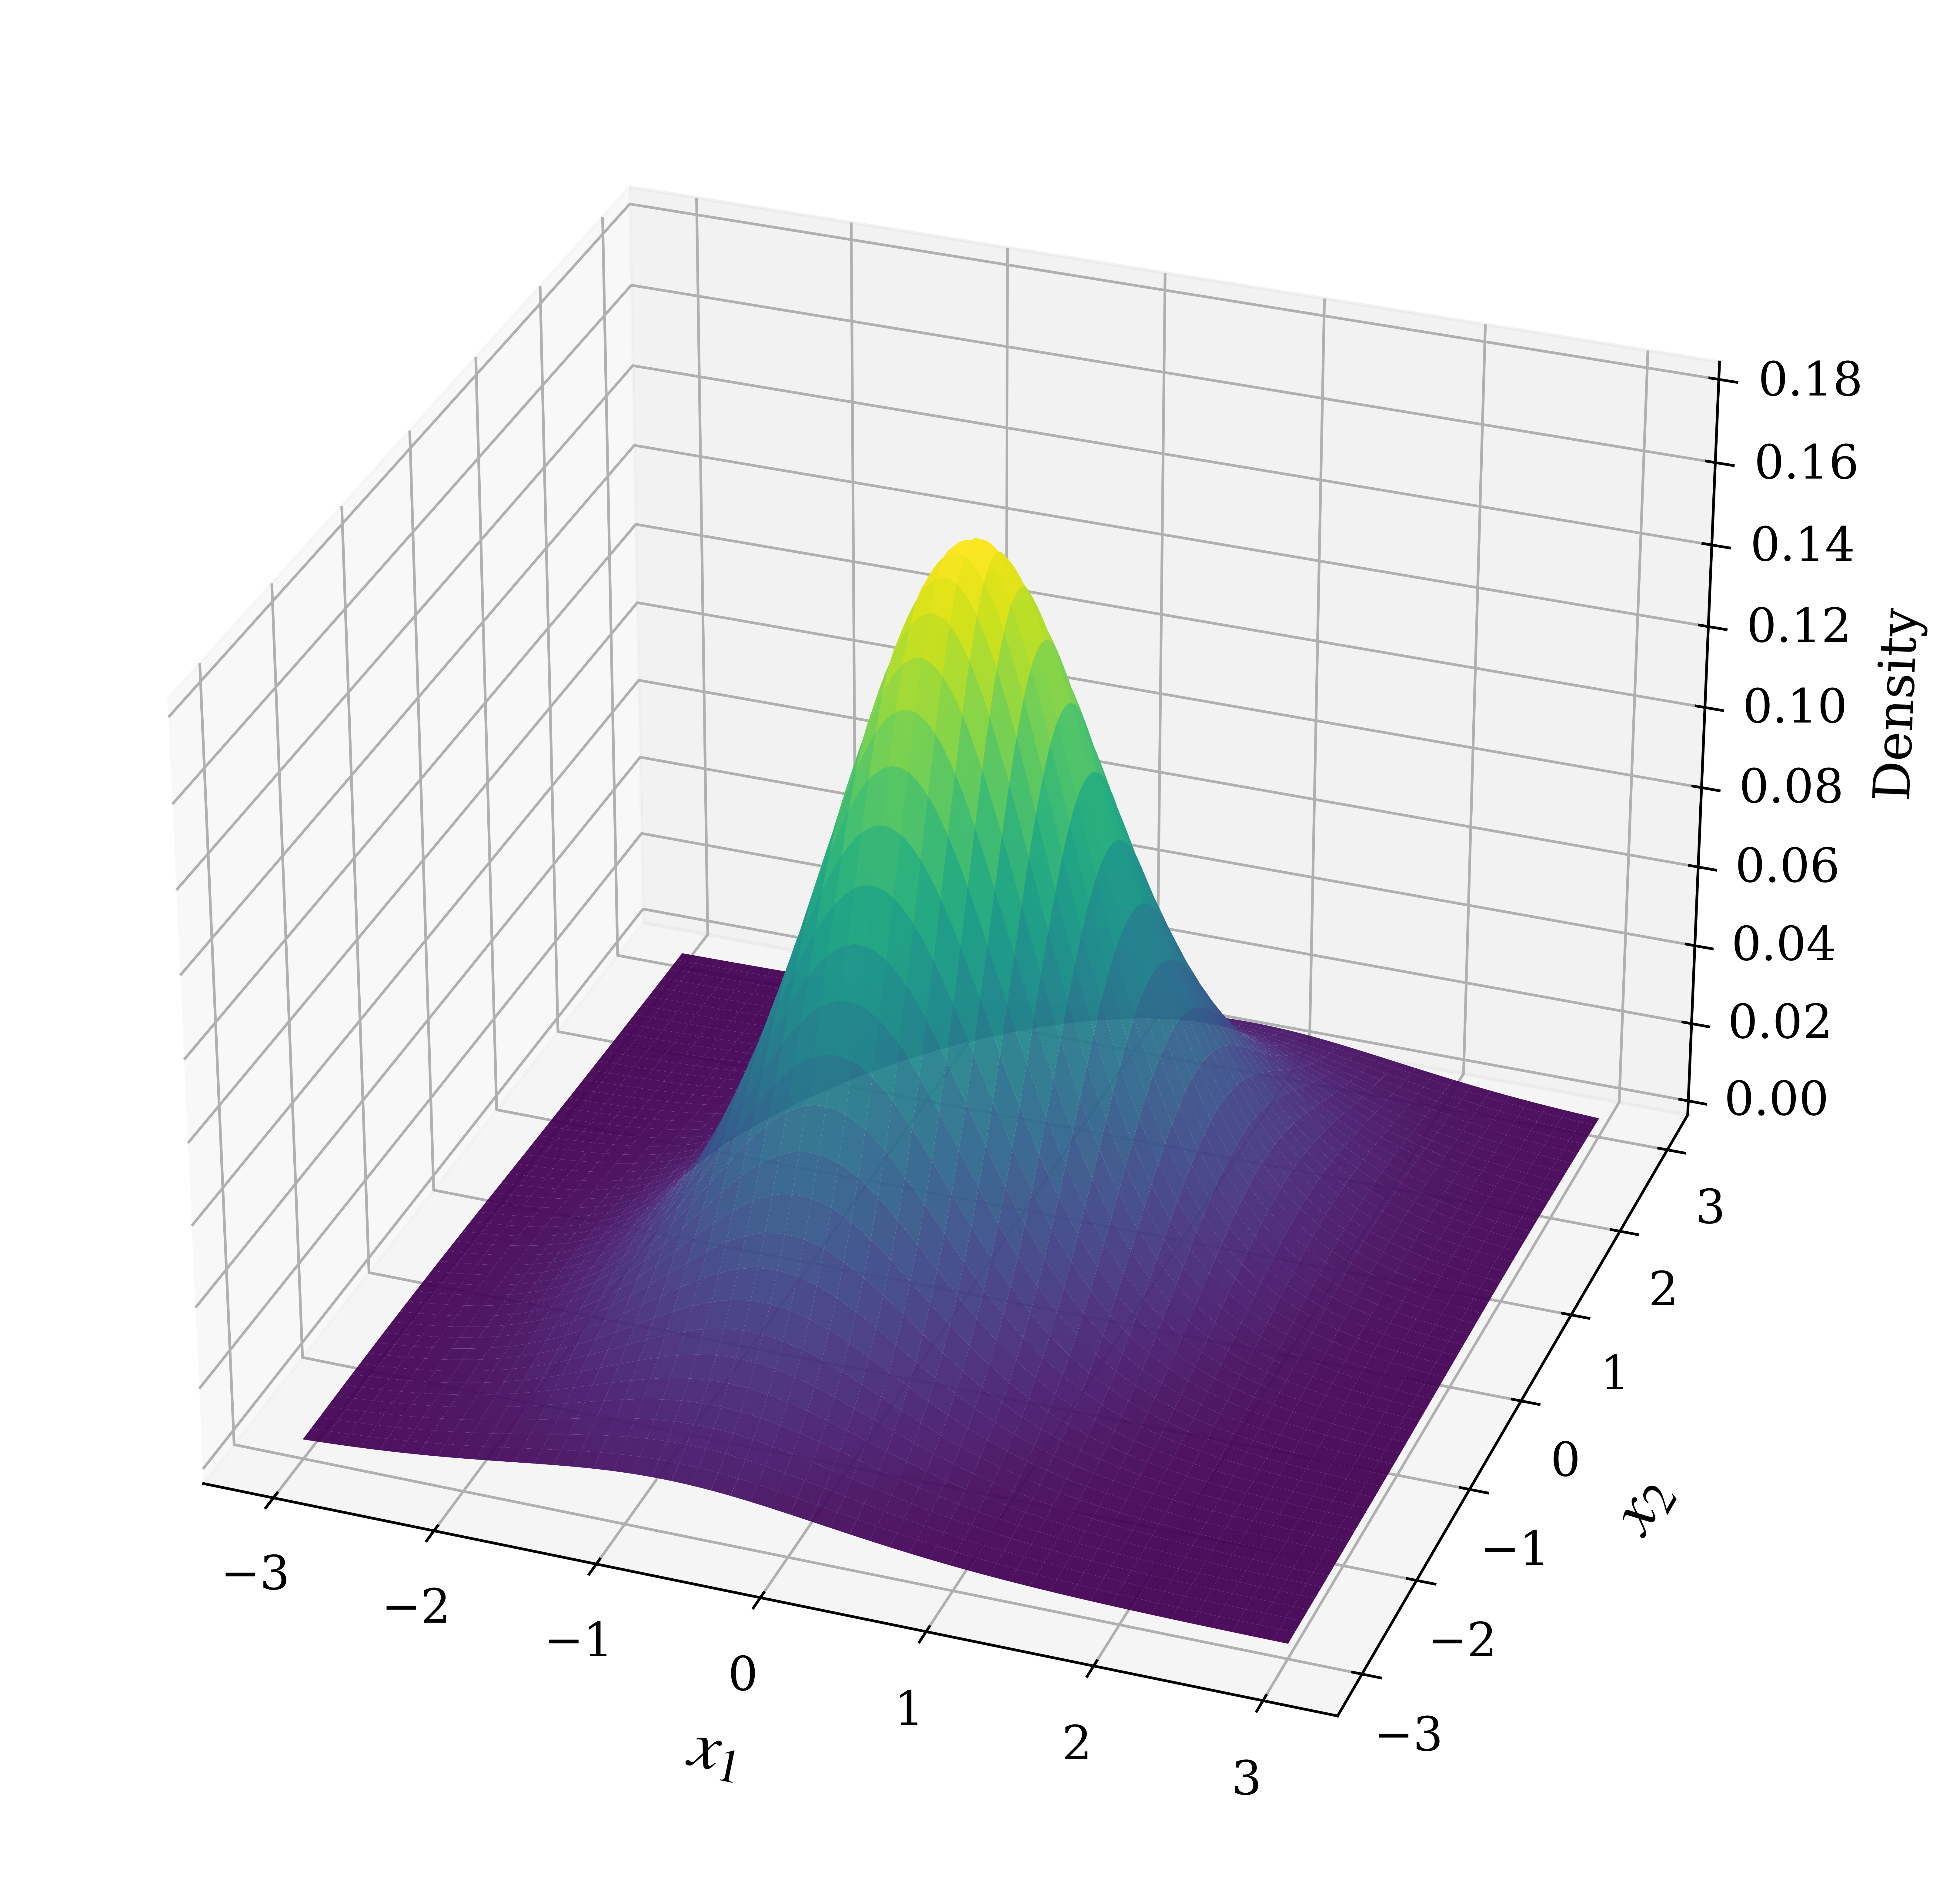
\includegraphics[width=0.5\linewidth]{figures/plot16.png}
    }
    \caption{$\;$ Density of $\RIGauN$ distribution with various parameter combinations.}
    \label{zyf.four.S.fig4}
\end{figure}

\subsubsection{Mean regression model and MLEs computation for $\RIGauN$}       % Section S1.4.2

Suppose that $\{\ibX_i\}_{i=1}^n \ind \mbox{RIGau-N}_d(\bmu_i, \bSi, \la)$ and $\Y{obs} = \{\ibx_i, \ibzi\}_{i=1}^n$ denote the observed data, we consider the following mean regression model
$$
    E(\ibX_i | \ibzi) = \bmu_i = \bB^\top \ibzi, \quad i = 1, \dots, n, 
$$
where $\ibzi = (z_{i1}, \dots, z_{iq})^\top$ is a $q$-dimensional vector of covariates for the $i$-th subject, the matrix of regression coefficients
\begin{eqnarray*}
    \bB = \left(
    \begin{array}{cccc}
        \be_{11} & \be_{12} & \cdots & \be_{1d} \\ 
        \be_{21} & \be_{22} & \cdots & \be_{2d} \\ 
        \vdots   & \vdots   & \ddots & \vdots   \\
        \be_{q1} & \be_{q2} & \cdots & \be_{qd}
    \end{array}
    \right),
\end{eqnarray*}
with $q \times d + d(d + 1) / 2 + 1 \le n$. Let $\bga = \{ \bB, \bSi, \bla\}$ be the parameter vector, the log-likelihood function of $\bga$ is
\begin{eqnarray*}
    \ell_4(\bga | \Y{obs}) &\sr{\rm (\ref{zyf.four.S1.6})}& -\frac{n(d + 1)}{2} \log(2\pi) - \frac{n}{2} \log|\bSi| + n\la + \frac{n}{2} \log\la \\ [2mm]
    && +\; \sum_{i=1}^n \log \int_0^\infty h_4(\tau | \ibx_i, \ibzi, \bga) \rd \tau,
\end{eqnarray*}
where 
$$
    h_4(\tau | \ibx_i, \ibzi, \bga) \teq \tau^\frac{d - 1}{2} \exp\left\{-\frac{1}{2}\left[\left( \left(\ibx - \bB^\top \ibzi \right)^\top \bSi^{-1} \left(\ibx - \bB^\top \ibzi \right) + \la \right) \tau + \frac{\la}{\tau} \right]\right\}.
$$
To calculate the MLEs of $\bga$, we utilize the N-EM algorithm. By computing the ndf
\begin{eqnarray*}
    g_4(\tau | \ibx_i, \ibzi, \bga) &\teq& \frac{h_4(\tau | \ibx_i, \ibzi, \bga)}{\int_0^\infty h_4(s | \ibx_i, \ibzi, \bga) \rd s} \\ [2mm]
    &=& \GIGau\left( \tau \;\bigg| \left(\ibx_i - \bB^\top\ibzi\right)^\top \bSi^{-1} \left(\ibx_i - \bB^\top \ibzi\right) + \la,\; \la,\; \frac{d + 1}{2}\right),
\end{eqnarray*}
we construct the surrogate function 
\begin{eqnarray*}
    Q_4(\bga | \bgat) &=& \ct{4} - \frac{n}{2} \log|\bSi| - \frac{1}{2} \sum_{i=1}^n \at{i,4} \left(\ibx_i - \bB^\top \ibzi \right)^\top \bSi^{-1} \left(\ibx_i - \bB^\top \ibzi \right) \\ [2mm]
    && +\; \frac{n}{2} \left[ \left(2 - \Bat{4} - \Bbt{4}\right) \la + \log\la \right],
\end{eqnarray*}
with constant $\ct{4}$ free from $\bga$ and for $i = 1, \dots, n$, 
\begin{eqnarray*}
    && \at{i,4} = \int_0^\infty \tau \cdot g_4(\tau | \ibx_i, \ibzi, \bgat) \rd \tau, \quad \Bat{4} \teq \frac{1}{n} \sum_{i=1}^{n} \at{i,4}, \\ [2mm]
    && \bt{i,4} = \int_0^\infty \frac{1}{\tau} \cdot g_4(\tau | \ibx_i, \ibzi, \bgat) \rd \tau, \quad \Bbt{4} \teq \frac{1}{n} \sum_{i=1}^{n} \bt{i,4}.
\end{eqnarray*}
By maximizing $Q_4(\bga | \bgat)$ respect to $\bga$, we obtain the $(t+1)$-th approximation of $\hbga$ as
\begin{eqnarray*}
    \bBtI &=& \left[ \sum_{i=1}^n \at{i,4} \ibzi \ibziT \right]^{-1} \left[ \sum_{i=1}^n \at{i,4} \ibzi \ibx_i^\top \right] = \left(\bZ^\top \At{4} \bZ\right)^{-1} \left(\bZ^\top \At{4} \bX\right), \\ [2mm]
    \bSitI &=& \frac{1}{n} \sum_{i=1}^n \at{i,4} \left( \ibx_i - \bB^{(t+1)\top} \ibzi\right) \left( \ibx_i - \bB^{(t+1)\top}\ibzi \right)^\top \\ [2mm]
    &=& \frac{1}{n}\left(\bX - \bZ \bBtI \right)^\top \At{4} \left(\bX - \bZ \bBtI \right), \\ [2mm]
    \latI &=& \left( \Bat{4} + \Bbt{4} - 2 \right)^{-1},
\end{eqnarray*}
where $\bZ = (\ibz_{(1)}, \dots, \ibz_{(n)})^\top$, $\At{4} = \diag(\at{1,4}, \dots, \at{n,4})$ and $\bX = (\ibx_1, \dots, \ibx_n)^\top$.